\label{kolmo_rbn_chapter}
In Section \ref{Applications_RBN}, some of the many different applications of the Boolean Networks were mentioned, especially, those for the Random Boolean Networks. These networks are useful to model and simulate networks that can be found in nature, but also in areas such as sociology, economics, computer science, etc. Hence, its study is important since they can be used to elucidate the hidden properties of these systems. Evidently, the capacity of a network to simulate a system depends on the topology and in the updating functions used. There are Boolean Networks which are more powerful than others. One indicator of the power of a Boolean Network must be its complexity. A network which is simple should not be able to imitate the behavior of complex networks such as the genetic regulatory ones. Nonetheless, the question of how to measure the complexity of a Boolean Network is not trivial. The main problem is that a Boolean Network is defined by two independent components, its topology, and its updating functions. These components then are brought together to create a dynamical system. This dynamical system is what we properly know as a Boolean Network and the object to which it is desirable to measure its complexity. Thus, measuring the complexity of its components separately may not be the best approach. We must devise a way to measure the complexity of both components acting together.\\

In this chapter, we will propose a way to measure the complexity of Boolean Networks. This proposal will be tested by using Random Boolean Networks. We will begin by measuring the complexity of random sequences of bits since they will be the key for measuring the complexity of Boolean Networks. Later, a procedure to measure the complexities of the individual components of a Boolean Network will be proposed. First, a method to measure the complexity of the topology will be studied. The topology is a directed graph, so this method will be tested firstly with graphs and then with digraphs. Afterward, the effect of the isomorphic representation used to represent the network will be studied. Next, a method to measure the complexity of the updating functions will be proposed. Finally, a method to measure the complexity of Boolean Networks will be presented and tested.
%poner y agregar más cosas como lo encerrado en rosa (pags 1 y 2) del art on measuring the complex of networks

\section{Software and Hardware Features}
To perform the experiments of this chapter, the implementation described in Section \ref{Library_K_complex} to measure Kolmogorov complexity will be used. Specifically, the implementation written in the Wolfram Language (Mathematica). This library contains the function \textit{StringBDM} which measures the complexity of sequences of bits. It accepts a string of $0's$ and $1's$ as input and returns the complexity computed by means of the Block Decomposition Method (BDM) with the help of short sequences for which K-complexity was computed by means of the Coding Theorem Method (CTM). It is possible to control the overlapping parameter of the method, though by default it is set to be $1$. We always will use the default parameter.\\

Additionally, this library contains the function \textit{BDM} which allows measuring the complexity of adjacency matrices. These matrices must be composed of only $0's$ and $1's$, and they are introduced to the function as a list of lists. This is the 2-D generalization of the original Block Decomposition Method. It uses the complexity computed by means of the CTM for square matrices with sizes ranging from $1 \times 1$ to $4 \times 4$. In this work, we will only use the $4 \times 4$ matrices to perform the 2-dimensional BDM.\\

In this chapter, every time we mention Kolmogorov complexity, K-complexity or algorithmic complexity, we are referring to the approximation computed by means of the Block Decomposition Method. The codes of this chapter were implemented in \textit{Mathematica 12} (version 12.0.0.0) in a 64-bits system with \textit{Windows 10}. 

\section{The Complexity of Random Sequences of Bits}
\label{complex_seqs_section}
We performed this first experiment to be sure that the implementation to measure Kolmogorov complexity works as expected and to gain some experience in its use. The idea is simple, we generate a given number of $1$-dimensional vectors of the same size. These vectors are initialized with zeros and we introduce them in a cycle. In the first iteration, we take the first of these vectors and we introduce it to another cycle (we have a nested cycle). In this nested cycle, we run over the indices of the vector, and with a probability $p$ we change the zero in each element of the vector by a one (the probability that we do not change the zero in each element is $1-p$). Once we have iterated through all the elements of the vector, we measure the Kolmogorov complexity of the resulting sequence. We also measure the Shannon entropy of the resulting sequence by means of the \textit{Entropy} built-in function of Mathematica and we compress it in $GZIP$ format to measure its file size. To better capture the complexity as a function of the parameter $p$, we repeat the process of replacing zeros by ones for each sequence $T$ times, measuring the Kolmogorov complexity, the entropy, and the file size each time. Finally, we compute the quartiles for each set of measurements and take the mean by only considering the second and third quartiles. This trimmed mean procedure eliminates possible fluctuations in the results which can be seen as noise \footnote{For instance, it is possible that although the parameter $p$ would have a high value like $0.9$, the sequence obtained can be almost full of zeros, even though it so unlikely. This method allows us to avoid this problem and better capture the complexity of the sequences as a function of $p$.}. We save the results.\\

Once we have finished, we take the second vector and repeat the same algorithm, however this time the probability of changing a zero by a one is $p+dp$. We do so until we have used all the vectors, summing $dp$ to the probability parameter in each iteration. Evidently, the parameter $p$ is such that $0\leq p \leq 1$. Therefore, we initialize $p=0$ and make sure that the number of vectors is such that to the last one will correspond the probability $p=1$, i.e., the first vector will be full of zeros, and the last one will be full of ones.\\

The result of two experiments is shown in Fig. \ref{fig:random_seqs}. We used sequences of length $100$ and $1000$. In both experiments, the step size in the probability was $dp=0.01$ and the number of random sequences generated with the same $p$ value was $10$, from which the trimmed mean described before was done. As expected, for short sequences the lossless compression method failed to describe the complexity of the sequences since we expected the sequences with $p=0$ and $p=1$, i.e., sequences full of zeros and ones, to have a complexity close to zero. Meanwhile, the entropy and Kolmogorov complexity had a quite similar performance. As can be seen, for longer sequences the behavior of the entropy was more like the lossless compression method, which means that compression algorithms describe better the complexity of long sequences. However, these two methods were far from the result given by Kolmogorov complexity which as we argued before must be a better measurement of complexity.\\

\begin{figure}
	\centering
	\begin{subfigure}[b]{0.49\textwidth}
		\centering
		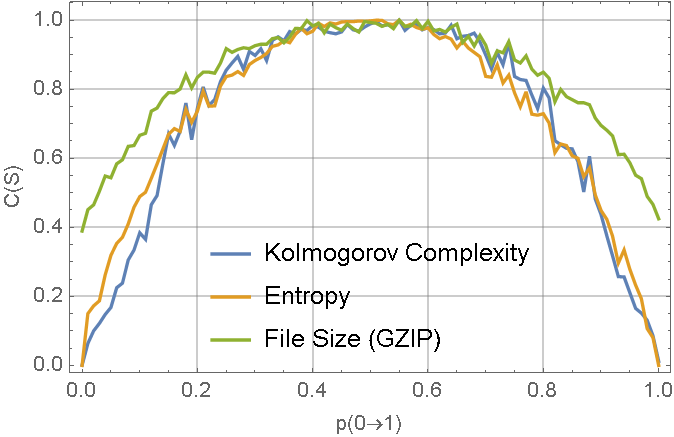
\includegraphics[width=\textwidth]{100_size_random_seqs}
		\caption{}
		\label{fig:100_size_random_seqs}
	\end{subfigure}
	%\hfill
	\hspace{0.5mm}
	\begin{subfigure}[b]{0.49\textwidth}
		\centering
		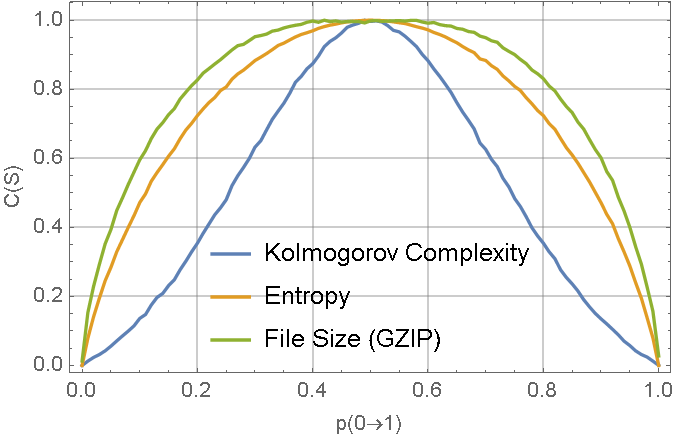
\includegraphics[width=\textwidth]{10000_size_random_seqs}
		\caption{}
		\label{fig:10000_size_random_seqs}
	\end{subfigure}
	\caption[Complexity measurements for random binary sequences with three different methods.]{Complexity measurements for random binary sequences with three different methods versus the probability of changing a $0$ by a $1$ in each element of the sequence. For purposes of comparison, the results have been normalized such that the maximum value in each method equals $1$. (a) Sequences of length $100$, (b) Sequences of length $10000$. See the text for more details.}
	\label{fig:random_seqs}
\end{figure}

Therefore, we can say that in general, lossless compression techniques are the worst, particularly for short sequences (around hundreds of bits). For short sequences, Shannon entropy has a similar performance to Kolmogorov complexity. Nevertheless, for long sequences (around thousands of bits) lossless compression techniques have more acceptable performance and their result is similar to that given by the entropy, although, both methods have a poor performance when compared with Kolmogorov complexity which we expect to be the nearest value to the true complexity value of the sequence, so we always should choose this method, especially for long sequences, leaving the use of entropy only for short sequences and avoiding if possible the lossless compression techniques. If we cannot measure Kolmogorov complexity, we always should try to use entropy over compression methods, especially for short sequences.\\

The code used to carry out this experiment can be found in the Appendix Section \ref{codes_wolfram} (Fig. \ref{fig:random_seqs_code}). A similar experiment with similar results was performed by \cite{decomposition} (section 6).

\section{The Complexity of Random Graphs}
\label{comp_graphs_section}
In this section, experiments regarding the complexity of random graphs will be presented. The main idea is to generate random graphs following a graph distribution. The complexity of the generated graphs is controlled by a parameter which can introduce order or disorder depending on its value. The experiments presented in this section are based on the work presented in \cite{kolmo_graph}.

\subsection{Complexity from The Watts-Strogatz Graph Distribution}
\label{Watts-Strogatz_section}
The first graph distribution which will be used to generate random graphs will be the Watts-Strogatz graph distribution. This graph distribution can be easily implemented in Mathematica by means of the built-in function \textit{WattsStrogatzGraphDistribution}. We described how this function works in Section \ref{Watts-Strogatz} and Fig. \ref{fig:strogatz_graphs}. A random graph is randomly chosen from this distribution using the built-in \textit{RandomGraph} function.\\

The algorithm is like that used for measuring the complexity of random sequences of bits. We use a cycle to generate random graphs. The complexity of each graph obtained is controlled by the parameter $p$, i.e., the probability of rewiring. The initial value of this parameter is $p=0$ and at each iteration, we increase its value using a probability step of size $dp$. The generation of graphs is stopped until we have reached the value $p=1$.\\

At each step, the complexity of the generated graphs is measured by using the adjacency matrix as a representation of each graph. This time, only the Kolmogorov complexity and the Shannon entropy methods are used, since as was seen in the former section, lossless compression techniques are no better than the entropy to describe complexity.  To do so, the adjacency matrix is flattened, i.e., we create a unique binary vector which contains the rows of the adjacency matrix one after the other. In this way, the complexity of each graph can be measured as usual, just by measuring the complexity of this binary sequence. Additionally, for purposes of comparison of this approach, we also used the 2D generalization of the BDM method which allows measuring directly the Kolmogorov complexity of adjacency matrices.\\

To eliminate fluctuations in the results, we also performed a trimmed mean procedure as we did for binary sequences, which means that we generate a given number of graphs using the same probability parameter $p$. Then, we measure their complexity and compute the quartiles of this set of results. Finally, the mean is computed by considering only the second and third quartiles.\\

As we saw in Fig. \ref{fig:strogatz_graphs}, graphs generated using the parameter value $p=0$ seem to be highly regular and thereby not complex. On the other hand, graphs with the parameter value $p=1$ seem to be highly random and thereby very complex. Intermediate $p$ values seem to have a complexity in between. Hence, we expect this experiment will show this complexity behavior as a function of the parameter $p$.\\

\begin{figure}
\centering
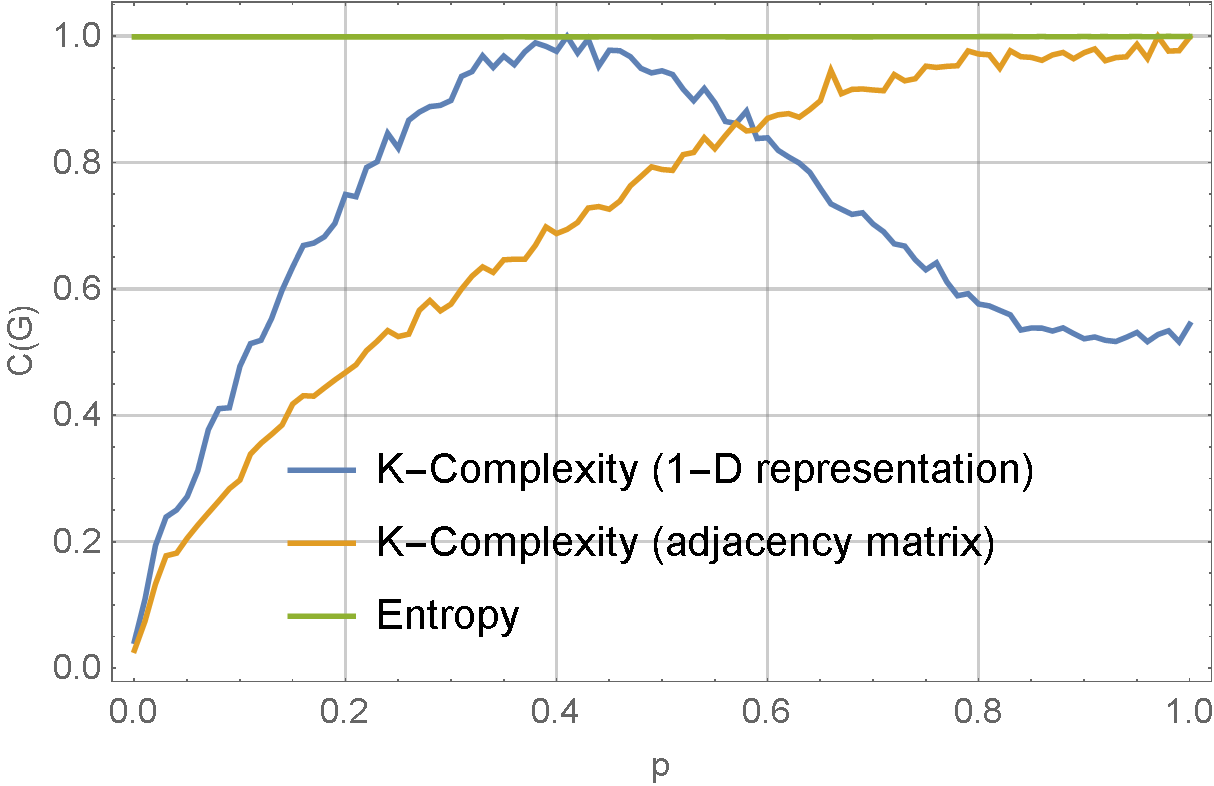
\includegraphics[width=\textwidth]{resultswatts}
\caption[Complexity measurements using three different methods of random graphs obtained from the Watts-Strogatz graph distribution.]{Complexity measurements using three different methods of random graphs obtained from the Watts-Strogatz graph distribution versus the probability parameter $p$. The graphs generated had $100$ nodes and were created starting from a $10$-regular graph following the Watts-Strogatz procedure. The number of random graphs generated with the same $p$ value was $10$ from which the trimmed mean described before was done. For purposes of comparison, the results obtained with each method were normalized with respect to the maximum value.}
\label{fig:resultswatts}
\end{figure}

The result of this experiment is shown in Fig. \ref{fig:resultswatts}. We can see that the results obtained by measuring the entropy of the 1-D representation of each graph remained practically constant, which means that this method is not capable of detecting changes in complexity by varying the parameter $p$. Meanwhile, the results obtained by measuring the Kolmogorov complexity with the 1-D representation had a better performance at the beginning, however, they reached its maximum approximately in $p=0.4$ and then the complexity value started to fall. On the other hand, the measurement of complexity using directly the adjacency matrix representation captured exactly the expected behavior of the complexity versus the parameter $p$, i.e., the complexity at $p=0$ is low and it increases until it reaches its maximum at $p=1$. This increasing seemed to follow a power-law $c(G) \sim p^{\alpha}$ with $0 < \alpha \leq 1$.\\

The code used to carry out this experiment can be found in the Appendix Section \ref{codes_wolfram} (Fig. \ref{fig:watts_code}).

\subsection{Complexity from The Barabási-Albert Graph Distribution}
\label{barabasi_experiment_text}
This experiment is almost the same as the former, but now we will use the Barabási-Albert graph distribution to generate random graphs. This distribution is implemented in Mathematica by means of the built-in function \textit{BarabasiAlbertGraphDistribution}. We have already described how this function works in Section \ref{Barabasi-Albert} and Fig. \ref{fig:albert_graphs}. As we mentioned before, this distribution is controlled by the parameter $k$, which is the number of edges of the vertex which is added at each step of the procedure.\\

According to Fig. \ref{fig:albert_graphs}, we expect that the complexity of these graphs will increase with the parameter $k$. However, this complexity must reach a maximum and start to fall from it as we continue increasing $k$, because for a sufficiently large value of $k$, the number of available nodes to link these $k$ edges will not be sufficient and we will end with the case where each node will be linked to every other node, i.e., we would get a complete graph which would be highly regular and symmetric, thus with a low complexity.\\

\begin{figure}
\centering
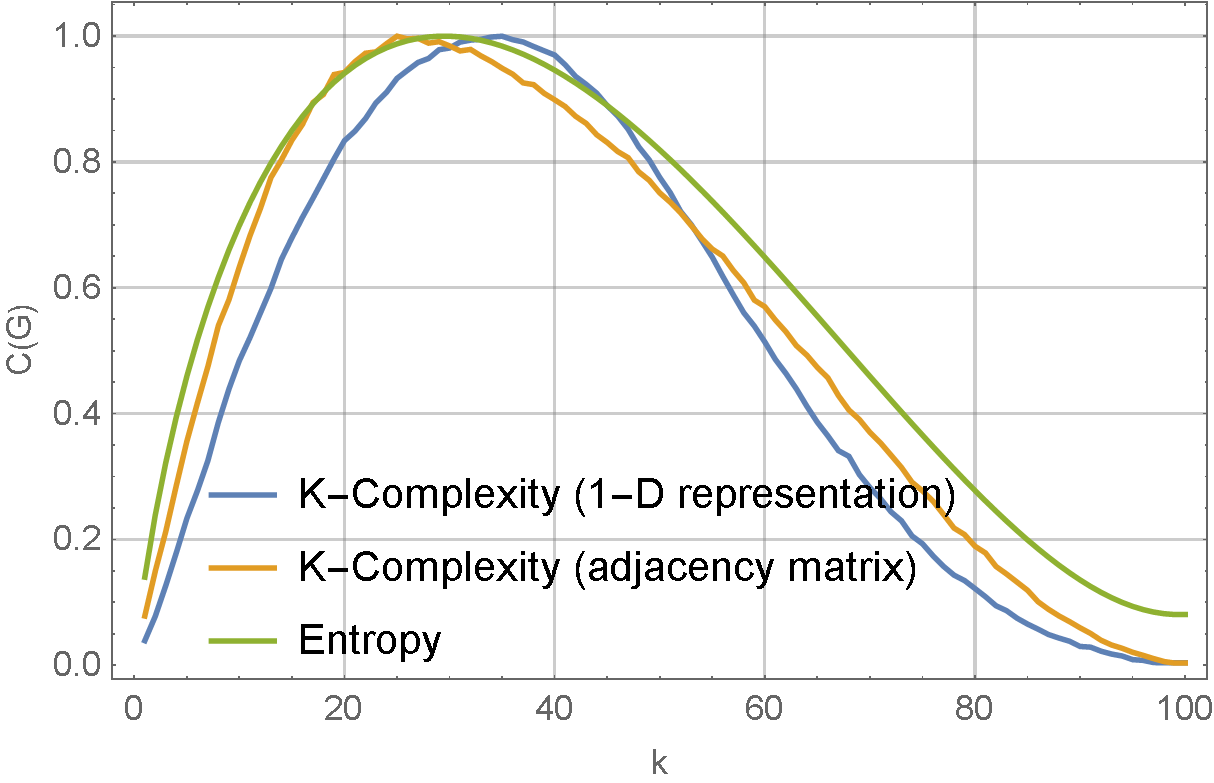
\includegraphics[width=\textwidth]{results_barabasi}
\caption[Complexity measurements using three different methods of random graphs obtained from the Barabási-Albert graph distribution.]{Complexity measurements using three different methods of random graphs obtained from the Barabási-Albert graph distribution versus the parameter $k$. The graphs generated had $100$ nodes and each one was created starting from a cycle graph of $3$ nodes following the Barabási-Albert procedure. The number of random graphs generated with the same $k$ value was $10$ from which the trimmed mean described before was done. For purposes of comparison, the results obtained with each method were normalized with respect to the maximum value.}
\label{fig:results_barabasi}
\end{figure}

The result of this experiment is shown in Fig. \ref{fig:results_barabasi}. As can be seen, the results showed the behavior expected by intuition. The complexity increased with the parameter $k$ and reached a maximum approximately around $k=30$ from which it began to fall. What was surprisingly in these experiments is that the results obtained using the three different methods to measure the complexity were very similar.\\

From the results obtained in this experiment and the former, we can see that entropy is not a robust measure of complexity since it had a good performance when using the Barabási-Albert graph distribution but when using the Watts-Strogatz graph distribution the results were awful. On the other hand, the results obtained by using K-complexity agree with our intuition about the complexity of graphs. Nonetheless, the performance obtained when using the traditional 1-dimensional K-complexity method seems still depend on the representation chosen for the graphs since when we tried to measure the complexity of a graph generated from the Watts-Strogatz graph distribution, we found that its performance can be a little different from expected, even though the 1-D representation used was lossless. Even so, with the Barabási-Albert graph distribution, our 1-D representation had no problems, so even though its performance is not as good as using directly the adjacency matrix representation, there exist objects which do not have an adjacency matrix representation, so for those objects we can rely on a 1-D lossless representation to measure its complexity.\\

The code used to carry out this experiment can be found in the Appendix Section \ref{codes_wolfram} (Fig. \ref{fig:barabasi_code}).

\section{The Complexity of Random Digraphs}
\label{complex_di_section}
Now, in this section, we will perform experiments like those shown before but now with directed graphs. We are interested in measuring the complexity of random digraphs because they serve as the topology for Random Boolean Networks whose complexity will be studied later. This time we will use a uniform digraph distribution. Nevertheless, we need to find a parameter or a way to verify that the complexity we are measuring makes sense.\\

If we simply use a uniform digraph distribution of $n$ nodes and $k$ edges, picking out a random digraph and measuring its complexity, then the digraph chosen can be complex or not since we do not know what to expect. Hence, to control the complexity of the digraphs chosen, our first approach is to gradually increase the vertex in-degree $ d^{-}$ of the nodes. Another option could have been increasing the number of nodes $n$, however, we consider that this approach lacks interest since it is obvious that for instance, any digraph of $50$ nodes will be more complex than any digraph of $20$ nodes, but it is not obvious if any digraph of $n$ with in-degree $ d^{-}=50$ is more complex than any other digraph of $n$ nodes with in-degree $ d^{-}=20$. On the other hand, the vertex out-degree $ d^{+}$ can take any value. This choice is also motivated because in Classical Random Boolean Networks the topologies are chosen with a fixed number of nodes $n$ with a fixed vertex in-degree $ d^{-}$ and a vertex out-degree $ d^{+}$ which can vary. In the same sense, the digraphs generated will be allowed to have loops, though parallel edges (pointing in the same direction) will not be allowed. Thus, strictly speaking, we should call them multidigraphs, but we will continue calling them just as digraphs for simplicity.

\subsection{The Complexity from Increasing the Vertex In-Degree}
\label{comp_incr_vert_in_section}
In this experiment, we will generate a random digraph of $n$ nodes and $d^{-}$ incoming directed edges, and as usual, at each iteration its complexity will be measured. To measure its complexity we will use the three same methods we use in the last section, i.e., we will measure the Kolmogorov complexity directly from the adjacency matrix representation of the digraph, but also a 1-dimensional lossless representation will be created by putting the rows of the adjacency matrix one after the other. Then, the entropy and K-complexity of this 1-D representation will be measured. The vertex in-degree $ d^{-}$ of the random digraphs will be increased at each iteration while vertex out-degree $ d^{+}$ can vary. A procedure of trimmed mean to reduce fluctuations in the results will be performed as before as well.\\

It is expected that as the vertex in-degree $ d^{-}$ is increased, the complexity of the digraphs also will increase. However, as happened with the experiment in Section \ref{barabasi_experiment_text}, this complexity must reach a maximum and start to fall. This should happen since the case where the vertex in-degree $ d^{-}$ equals the number of nodes and therefore also the vertex out-degree ($ d^{-}=d^{+}=n$) is highly regular and symmetric, and thus with low complexity.\\

\begin{figure}
\centering
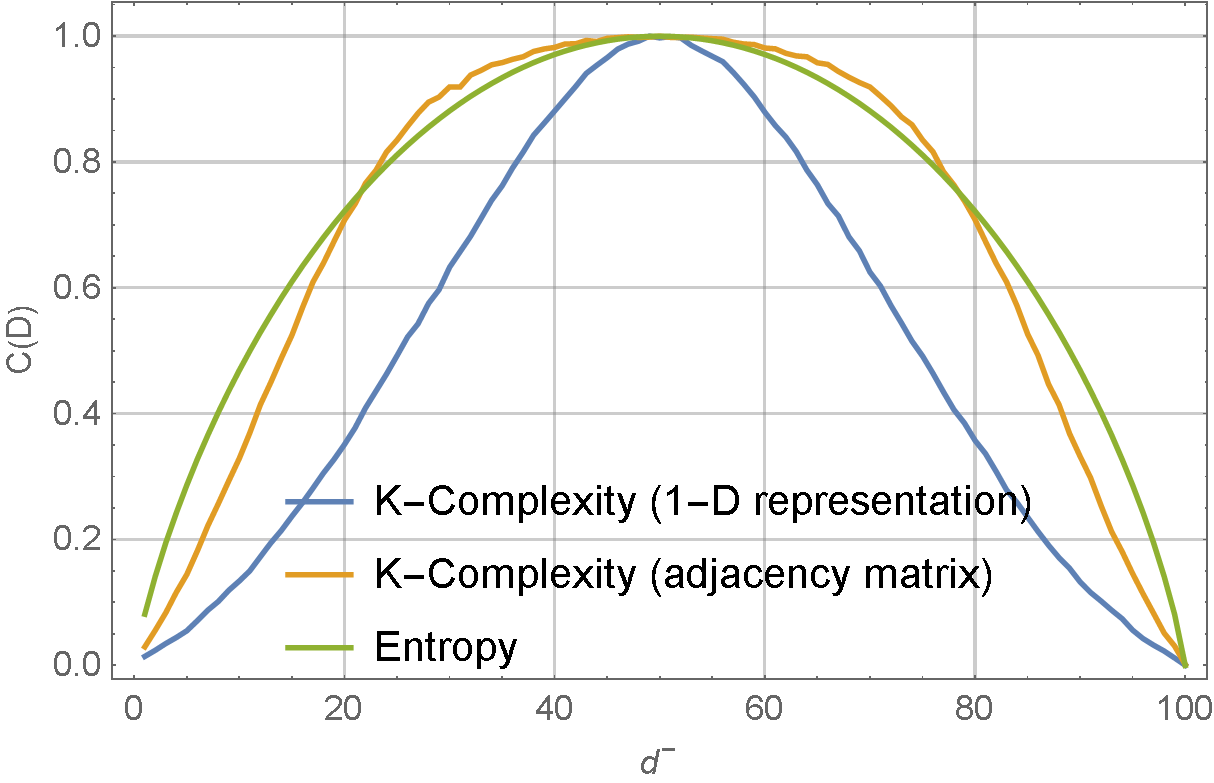
\includegraphics[width=\textwidth]{results_D_aum_d}
\caption[Complexity measurements using three different methods of random digraphs obtained from a uniform digraph distribution.]{Complexity measurements using three different methods of random digraphs obtained from a uniform digraph distribution versus the number of incoming directed edges $d^{-}$. The digraphs generated had $100$ nodes and the parameter $d^{-}$ was vary from $1$ to $100$. The number of random digraphs generated with the same $d^{-}$ value was $10$ from which the trimmed mean described before was done. For purposes of comparison, the results obtained with each method were normalized with respect to the maximum value. Compare these results with those shown in Fig. \ref{fig:10000_size_random_seqs}.}
\label{fig:results_D_aum_d}
\end{figure}

The result of this experiment is shown in Fig. \ref{fig:results_D_aum_d}. As can be seen, these results were very similar to the results of the experiment with random binary sequences (Fig. \ref{fig:10000_size_random_seqs}). In that experiment, we saw how Kolmogorov complexity had a better performance, showing a characteristic shape on its curve which could not be imitated by the entropy or compression techniques. If we now try to find this characteristic curve shape in the results in Fig. \ref{fig:results_D_aum_d}, we find that it is achieved by the Kolmogorov complexity measurement of our 1-D lossless representation. This is astonishing, considering that in the former experiments with graphs the adjacency matrix representation had a slightly better performance. This means that for directed graphs the lossless 1-dimensional representation we have proposed works better capturing the changes in complexity than the adjacency matrix representation, which this time gives results very similar to the entropy. Nevertheless, the three methods were able to show the behavior of the complexity that we expected, i.e., there is a maximum value in the complexity which in this case is found just in the middle ($d^{-}=50$) from which the complexity starts to fall, moreover, the curve is symmetric around this point.\\

From this experiment, we can conclude that the 1-D lossless representation we have proposed works better to describe the features which make a digraph to be complex or not through the Kolmogorov complexity.\\

This time the random digraphs were not generated by using a built-in function because Mathematica does not have any function which can be used to generate random digraphs with a given vertex in-degree $ d^{-}$, so we had to create our own algorithm to do so. The code used to carry out this experiment can be found in the Appendix Section \ref{codes_wolfram} (Fig. \ref{fig:direc_aum_d_code}).

\subsection{The Complexity from The Uniform Digraph Distribution}
\label{uni_di_dist_section}
In spite of the results obtained in the last experiment, they still not being so interesting if we wish to characterize not only the complexity of digraphs but also the complexity of the topology of Random Boolean Networks. In this model, both parameter $n$ and $ d^{-}$ remain fixed, so we would like to also maintain fixed these parameters and see the behavior in the complexity of random directed graphs in this way. However, once we maintain fix these parameters, we will not be able to control the complexity of the networks, so the results just will fluctuate, and it will be impossible to infer anything about its behavior. To solve this problem, we designed the following approach.\\

We will generate random digraphs in the same exact way we did before, but now with both parameters, $n$ (number of nodes) and $ d^{-}$ (vertex in-degree) maintained fixed. The complexity of them will be measured using the exact same procedure we did in the former experiment. Then, once we have the results, they will be ordered in increasing order of complexity and some of the digraphs will be drawn. In this way, it should be possible to visualize characteristics which we expect make the digraphs to be complex or not, like symmetries or regularities.\\

Hence, the purpose of this experiment is to verify that the measurements of complexity of digraphs that we perform agree with our visual intuition of what should be considered as complex or not, especially in the extreme cases, just as we easily can say that the sequence $100101011$ is more complex than the sequence $111110000$.\\

\begin{figure}
	\centering
	\begin{subfigure}[b]{0.7\textwidth}
		\centering
		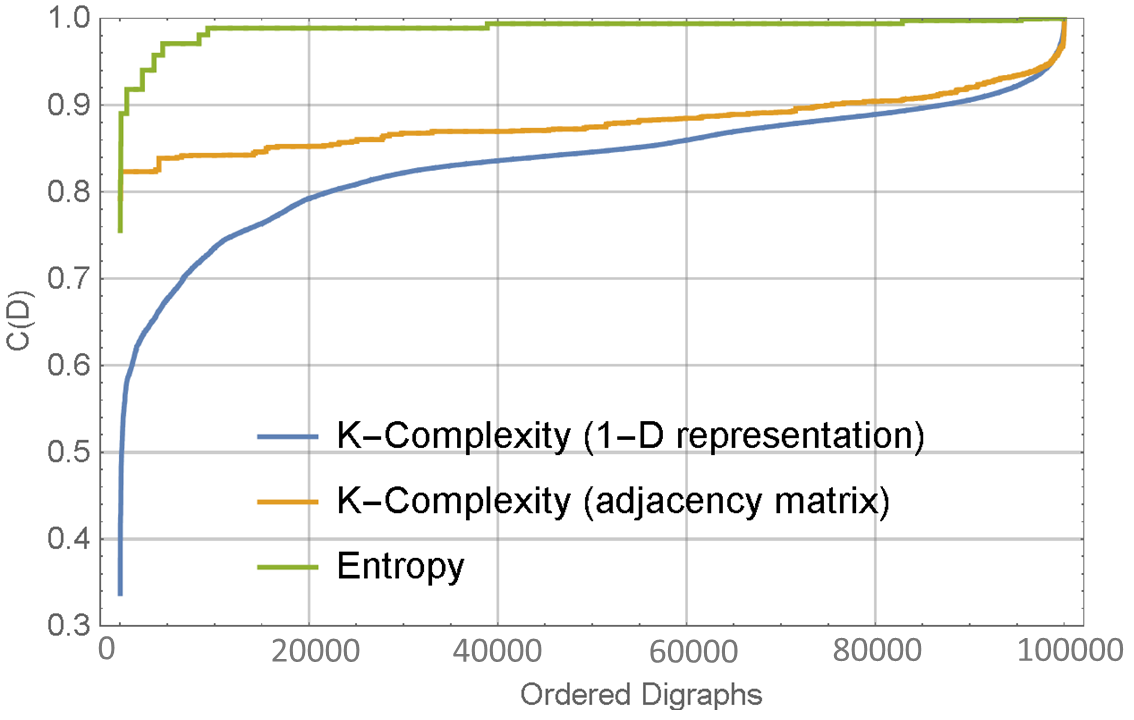
\includegraphics[width=\textwidth]{results_ordered_di_corrected}
		\caption{}
		\label{fig:results_ordered_di}
	\end{subfigure}
	%\\	
	\hfill
	%\hspace{0.5mm}
	\begin{subfigure}[b]{0.7\textwidth}
		\centering
		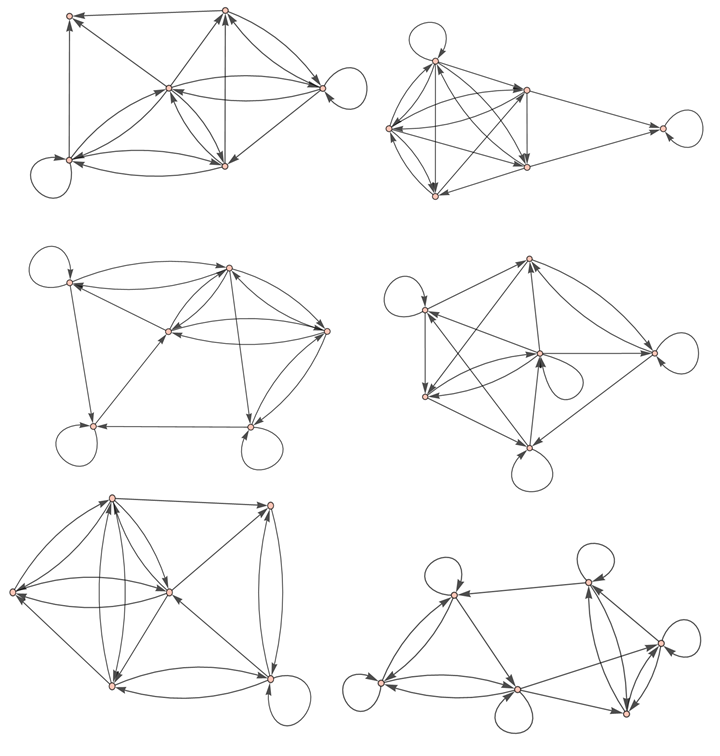
\includegraphics[width=\textwidth]{digraphs_increasig_complexity}
		\caption{}
		\label{fig:digraphs_increasig_complexity}
	\end{subfigure}
	\caption[Complexity measurements for random digraphs.]{(a) Complexity measurements for random digraphs. The results were ordered by increasing complexity value. The number of random digraphs generated was $100,000$ and all they had $6$ nodes and vertex in-degree $3$. For purposes of comparison, the results obtained with each method were normalized with respect to the maximum value. (b) Some directed graphs plotted by increasing complexity value. The complexity increases from left to right and from up to down. The order was obtained from the complexity measurements from the K-complexity method using a 1-D representation. The digraphs plotted were chosen from regular intervals of complexity, such that the digraph at the upper left corner is the less complex and the digraph at the lower right corner is the most complex digraph generated in the experiment.}
	\label{fig:digraphs_increasig_complexity_results}
\end{figure}

The result of this experiment is shown in Fig. \ref{fig:digraphs_increasig_complexity_results} and the code used can be found in the Appendix Section \ref{codes_wolfram} (Fig. \ref{fig:complex_di_k_cte_code}). As can be seen in Fig. \ref{fig:results_ordered_di}, the complexity for random digraphs with fixed parameters $n$ and $ d^{-}$ was bounded and did not vary much with the methods of entropy and K-complexity with an adjacency matrix representation. The method which again seemed to have better performance is the K-complexity with our 1-dimensional representation since it captured a much rich amount of complexity values, which means it can detect slight changes in complexity which the other methods cannot. This confirmed our previous observation that this method is better to describe the complexity of digraphs.\\

Since the measure of complexity with the K-complexity method and a 1-D representation increases gradually, it should be possible to reaffirm the difference between the complexity of extreme cases by using the visual representation, although due to the low variation in the values this could be no possible to do for intermediate cases, where the slope of the curve is not so high.  This is exactly what is shown in Fig. \ref{fig:digraphs_increasig_complexity}. For digraphs with intermediate complexity, it is hard to try to guess which one is more complex, however, for extreme cases, the situation is not as expected. For example, between the most complex and the less complex digraphs shown in Fig. \ref{fig:digraphs_increasig_complexity}, the difference in complexity is yet not clear, even though their computed complexities say there is a big difference.\\

A possible explanation for the above results is that we are not considering isomorphisms when measuring the complexity of the digraphs, i.e., the complexity of the digraph could be affected by the order the nodes are labeled since labeling the nodes in a different order gives a different representation of the object. Hence, it is possible that measuring the complexity of random digraphs is not enough and it is also needed to consider the complexity of its isomorphisms. In the next section, we will try to answer this question.

\section{The Complexity of Isomorphic Networks}
\label{comp_iso_net_section}
In this section, we will try to answer whether for the same graph or digraph the complexity measurement depends on the isomorphic representation used. First, an experiment using graphs will be performed followed by an experiment using digraphs.

\subsection{The Complexity of Isomorphic Graphs}
The experiment is quite simple. A random graph with a given number of nodes $n$ and a given number of edges $k$ will be generated by means of a uniform graph distribution which is easily implemented in Mathematica by means of the integrated function \textit{UniformGraphDistribution}. Then, the rows and columns of the adjacency matrix of the randomly generated graph will be permuted such that this process corresponds to a reorder in the labeling of the nodes, e.g., if the nodes of a graph are labeled as $\{1,2,3,4\}$ this process will permute the labels to a different order as can be $\{3,4,1,2\}$ or $\{4,3,2,1\}$. Clearly, the number of possible permutations in the labeling order of the $n$ nodes is $n!$. Thus, as the number of permutations increases fast for large networks, in general, it will not possible to use all the possible permutations. Therefore, we will work with a fixed number of permutations randomly chosen from a uniform distribution containing all the possible permutations. If two or more permutations are repeated, we will simply ignore these repetitions. To measure the complexity of the isomorphisms we will use the same three methods which we have been using lately.\\

\begin{figure}
	\centering
	\begin{subfigure}[b]{0.49\textwidth}
		\centering
		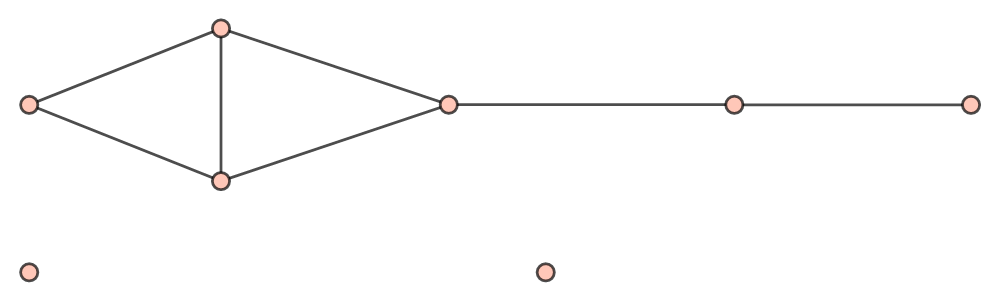
\includegraphics[width=\textwidth]{Grafo_iso_exp}
		\caption{}
		\label{fig:Grafo_iso_exp}
	\end{subfigure}
	%\hfill
	\hspace{0.5mm}
	\begin{subfigure}[b]{0.49\textwidth}
		\centering
		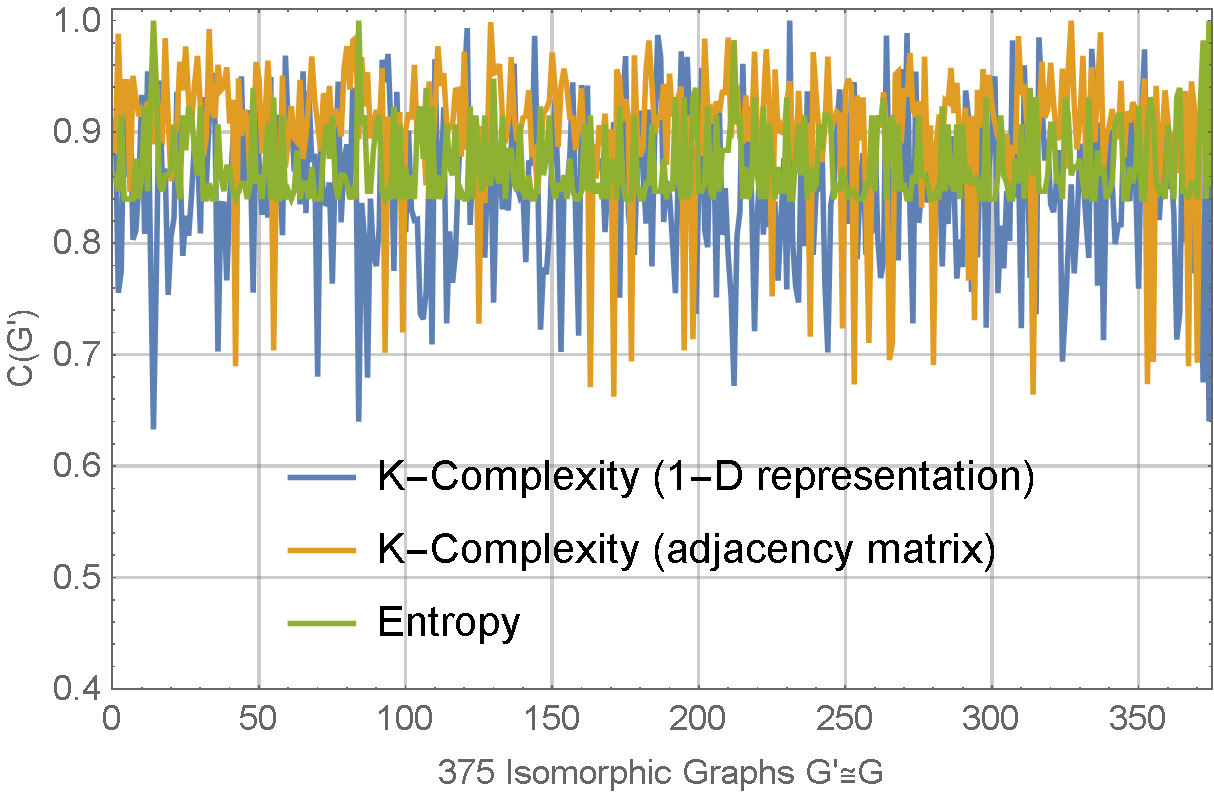
\includegraphics[width=\textwidth]{results_isoG}
		\caption{}
		\label{fig:results_isoG}
	\end{subfigure}
	\caption[Complexity measurements for isomorphic graphs.]{Complexity measurements for isomorphic graphs. (a) The random graph of $8$ nodes and $7$ edges for which the isomorphisms were generated. (b)Results obtained from measuring the complexity of the same graph with different isomorphic representations. The number of random permutations in the labels of the nodes used to generate the isomorphisms was $400$, but only the $375$ which were not repeated were considered. For purposes of comparison, the results obtained with each method were normalized with respect to the maximum value.}
	\label{fig:iso_G_complex_results}
\end{figure}

The result of this experiment is shown in Fig. \ref{fig:iso_G_complex_results} and the code used can be found in the Appendix Section \ref{codes_wolfram} (Fig. \ref{fig:iso_G_code}). As can be seen, the complexity of the same graph fluctuated depending on the order we labeled the nodes, i.e., which isomorphism was used to measure the complexity. This result is astonishing and at first, it was not expected since the Kolmogorov complexity had shown to be robust to different representations (see \cite{kolmo_graph}). However, this experiment proved that it is not robust for isomorphic graphs. Therefore, when trying to measure the complexity of a graph it is imperative to also consider its isomorphisms. According to the ideas of algorithmic complexity theory, which we reviewed in Chapter \ref{algorithmic_complexity_chapter}, the true Kolmogorov complexity must be the complexity obtained with the representation which gives the minimum value. Evidently, the Shannon entropy method also is subjected to this problem.\\

\begin{figure}
\centering
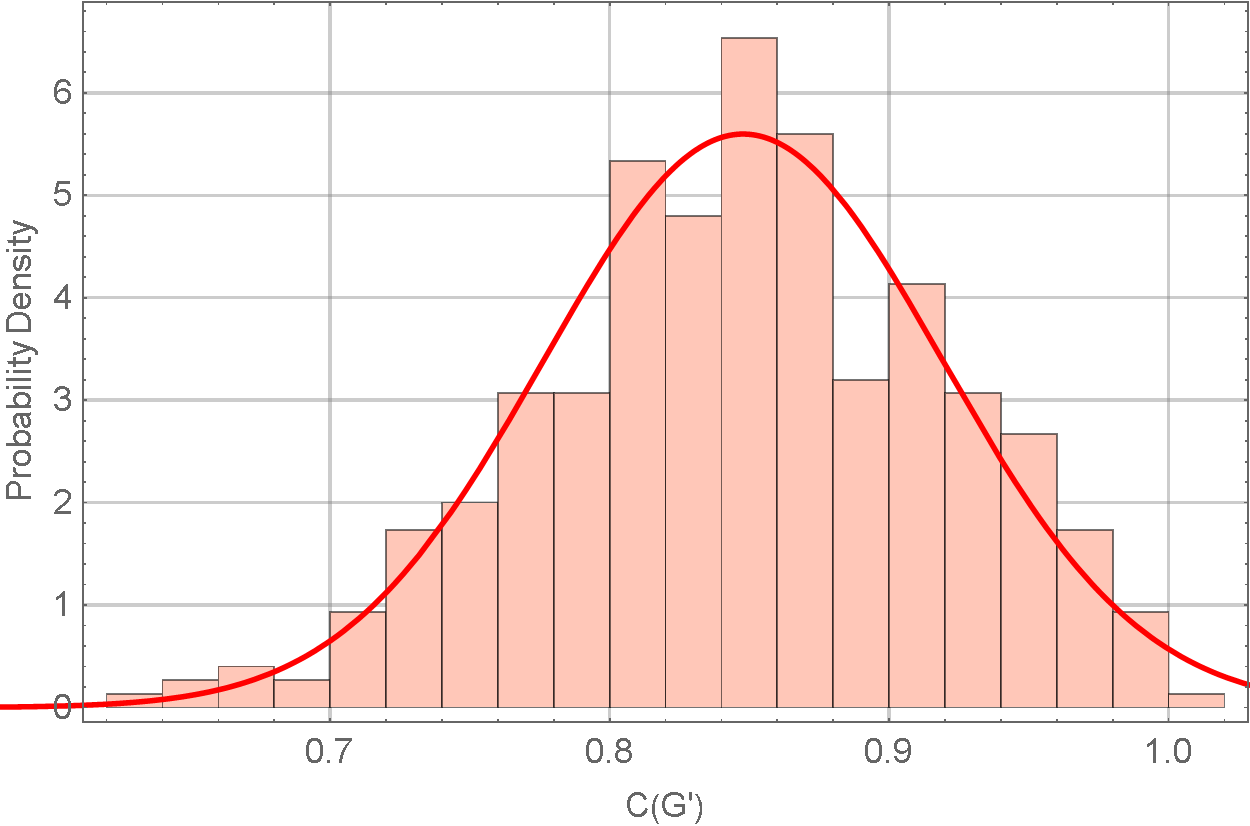
\includegraphics[width=\textwidth]{iso_G_prob_dist}
\caption[The distribution of complexities for the isomorphisms of a graph.]{The probability distribution which best fits the data shown in Fig. \ref{fig:results_isoG} (K-complexity of the 1-D representation). The distribution found is a normal distribution with parameters $\mu =0.847$ and $\sigma =0.071$.}
\label{fig:iso_G_prob_dist}
\end{figure}

As was mentioned, for large graphs with many nodes, the number of isomorphisms increases fast and becomes impractical to try to find the representation with the minimum value of complexity. Therefore, we would like to know if given a graph, is there a complexity value which is more probable to measure? Or in other words, we are interested in knowing the distribution of complexities for the isomorphisms of a given graph. Thus, we used the results of the experiment in Fig. \ref{fig:results_isoG} and with the help of the built-in function \textit{FindDistribution} of Mathematica we found the probability distribution which best fitted the data. The distribution fitted is shown in Fig. \ref{fig:iso_G_prob_dist}. This distribution is a normal distribution with parameters $\mu =0.847$ and $\sigma =0.071$. Therefore, the most probable value for the complexity of the graph shown in Fig. \ref{fig:Grafo_iso_exp} when choosing a random isomorphism was $\mu =0.847$ and the probability of measuring a complexity value in the interval $[- \sigma + \mu , \sigma + \mu]$ was $68.2 \%$.\\

\subsection{The Complexity of Isomorphic Digraphs}
Now, the former experiment will be repeated, but this time instead of a random graph, a random digraph of $n$ nodes and $k$ edges will be generated. The process to generate it will be again through the built-in function \textit{Random Graph} of Mathematica, but this time the option \textit{DirectedEdges $\rightarrow$ True} will be used to indicate that the $k$ edges must be directed. Then, the same procedure used before will be used to generate the isomorphisms, i.e., a fixed number of random permutations will be used to permute the order of the labels of the nodes. Finally, the complexity of the isomorphisms will be measured by using the three methods we have been implementing.\\

\begin{figure}
	\centering
	\begin{subfigure}[b]{0.49\textwidth}
		\centering
		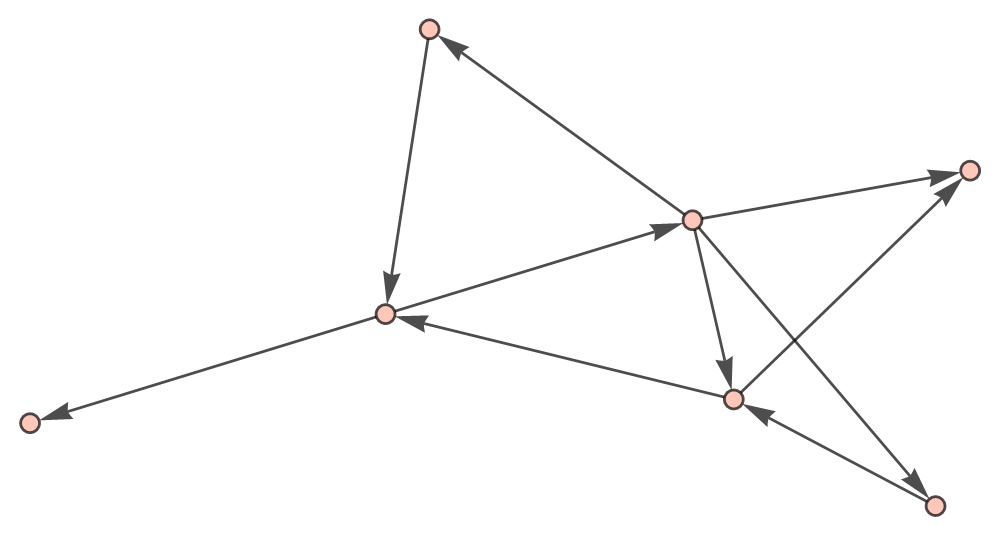
\includegraphics[width=\textwidth]{digafo_iso_exp}
		\caption{}
		\label{fig:digafo_iso_exp}
	\end{subfigure}
	%\hfill
	\hspace{0.5mm}
	\begin{subfigure}[b]{0.49\textwidth}
		\centering
		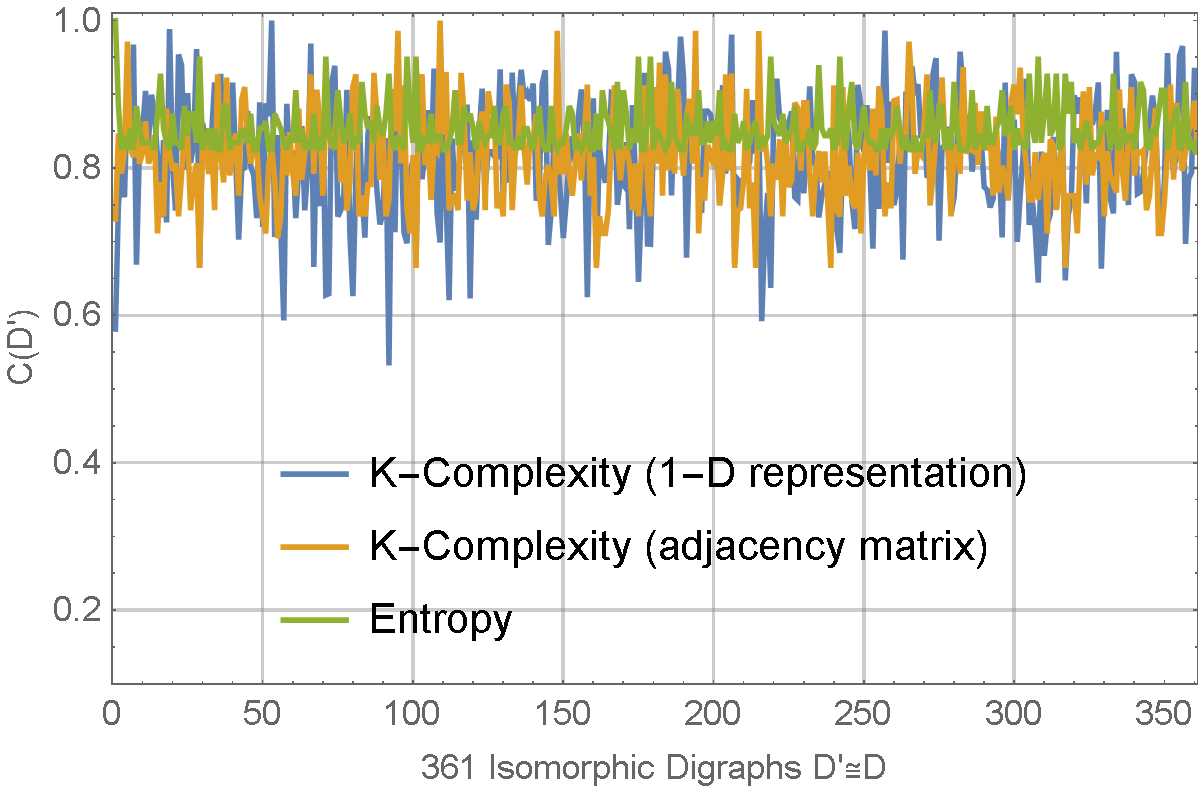
\includegraphics[width=\textwidth]{results_isoD}
		\caption{}
		\label{fig:results_isoD}
	\end{subfigure}
	\caption[Complexity measurements for isomorphic digraphs.]{Complexity measurements for isomorphic digraphs. (a) The random digraph of $7$ nodes and $10$ directed edges for which the isomorphisms were generated. (b)Results obtained from measuring the complexity of the same digraph with different isomorphic representations. The number of random permutations in the labels of the nodes used to generate the isomorphisms was $500$, but only the $361$ which were not repeated were considered. For purposes of comparison, the results obtained with each method were normalized with respect to the maximum value.}
	\label{fig:iso_D_complex_results}
\end{figure}

The result of this experiment is shown in Fig. \ref{fig:iso_D_complex_results} and the code used can be found in the Appendix Section \ref{codes_wolfram} (Fig. \ref{fig:iso_G_code}). The results showed, as they did for graphs, that the complexity of the digraphs also depends on the isomorphic representation used to measure its complexity. The fluctuations indicated that there are isomorphisms which representation gives a low complexity value while others give a high complexity value no matter what method was used to measure the complexity. Therefore, following the ideas of algorithmic complexity, the true complexity value must be that obtained with the isomorphic representation which gave the lower value.\\

\begin{figure}
\centering
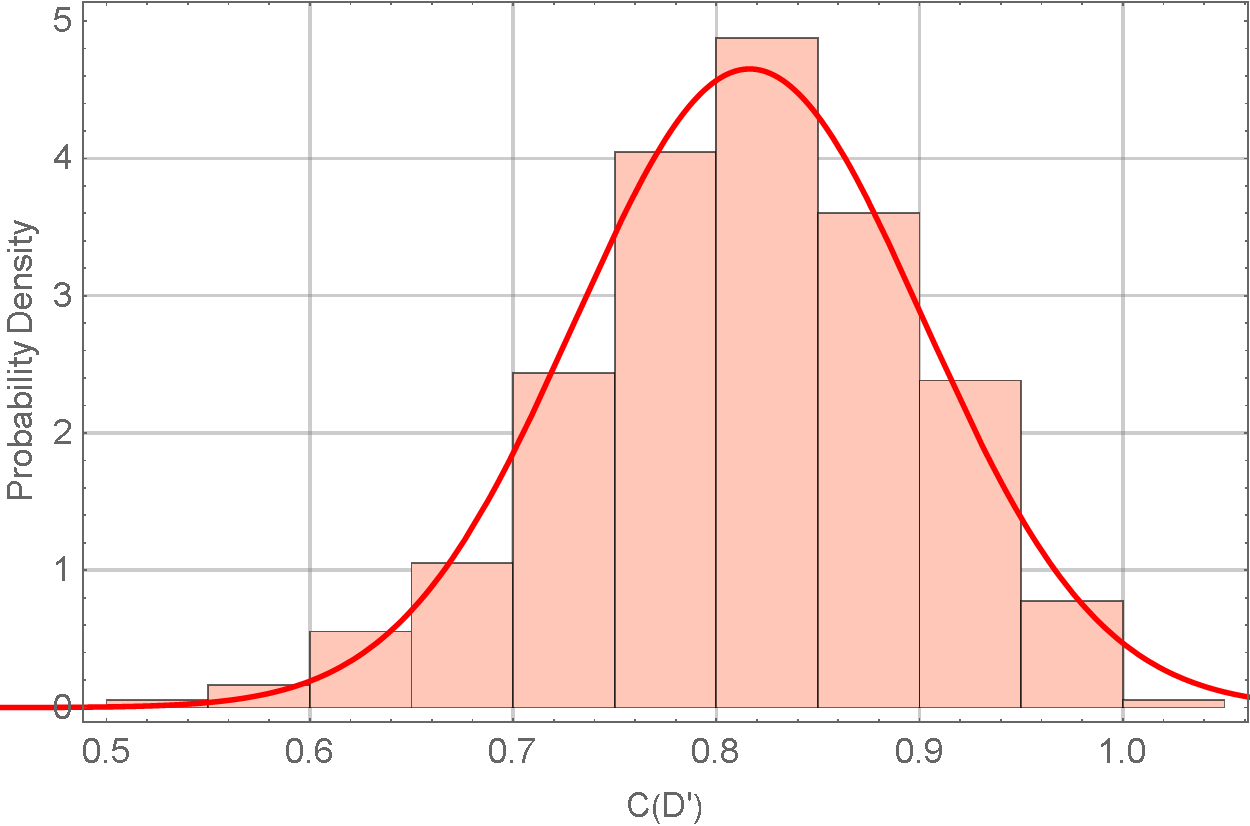
\includegraphics[width=\textwidth]{iso_D_prob_dist}
\caption[The distribution of complexities for the isomorphic representations of a digraph.]{The probability distribution which best fits the data shown in Fig. \ref{fig:results_isoD} (K-complexity of the 1-D representation). The distribution found is a normal distribution with parameters $\mu =0.816$ and $\sigma =0.085$.}
\label{fig:iso_D_prob_dist}
\end{figure}

Besides, as was did for isomorphic graphs, the distribution of complexities obtained using different isomorphic representations of the same digraph was calculated. The distribution which best fits the data in Fig. \ref{fig:results_isoD} was found using the function \textit{FindDistribution} of Mathematica. This distribution is shown in Fig. \ref{fig:iso_D_prob_dist}. Once more the distribution which best fitted the distribution of the complexities obtained by means of isomorphic representations was a normal distribution. This time the parameters of the distribution were $\mu =0.816$ and $\sigma =0.085$. Thus, the most probable value for the complexity of the digraph shown in Fig. \ref{fig:digafo_iso_exp} when choosing a random isomorphic representation was $\mu =0.816$ and evidently the probability of measuring a complexity value in the interval $[- \sigma + \mu , \sigma + \mu]$ again was $68.2 \%$ since this is a property of the normal distribution.\\

From this experiment and the former experiment with isomorphic graphs, we can conclude that the complexity measurement of a network depends on the specific isomorphic representation chosen to describe it. According to the ideas of algorithmic complexity, the true complexity of the network is the value obtained with representation which gives the lower complexity. Nonetheless, the number of isomorphisms increases fast with the number of nodes, so sometimes it will be impossible to tests all the isomorphism to find this true distribution. Fortunately, the distributions found in Figs. \ref{fig:iso_G_prob_dist} and \ref{fig:iso_D_prob_dist} are unimodal and show that there is a value of the complexity which is most probable to get when using any isomorphism and the probability of getting another value is not so high. Hence, even if not all the isomorphisms can be tested, we can use the most probable value of the distribution as an approximation of the complexity when comparing the complexities of many networks.

\subsection{The Complexity from The Uniform Digraph Distribution Revisited by Considering Isomorphisms}
\label{uni_di_dist_section_with_iso}
Coming back to the experiment about the complexity of random digraphs from the uniform digraph distribution (section \ref{uni_di_dist_section}), we found in Fig. \ref{fig:digraphs_increasig_complexity_results} that the random digraphs ordered by increasing value of complexity do not seem to show the same complexity increase when they are drawn. We expected a clear visual difference between the most complex digraph and the less complex digraph; however, this did not happen. That result took us to think we should consider the isomorphisms when measuring the complexity of digraphs. Now we have shown that this idea was correct, thus, the experiment of Section \ref{uni_di_dist_section} will be repeated, but now every time a random digraph is generated, also some of its isomorphisms will be generated and its complexity will be computed. As was argued before, the true complexity of the digraph must be the lower value obtained among the complexity values of the isomorphisms, so this criterion will be applied with the three methods to measure the complexity we have been using.\\

\begin{figure}
	\centering
	\begin{subfigure}[b]{0.65\textwidth}
		\centering
		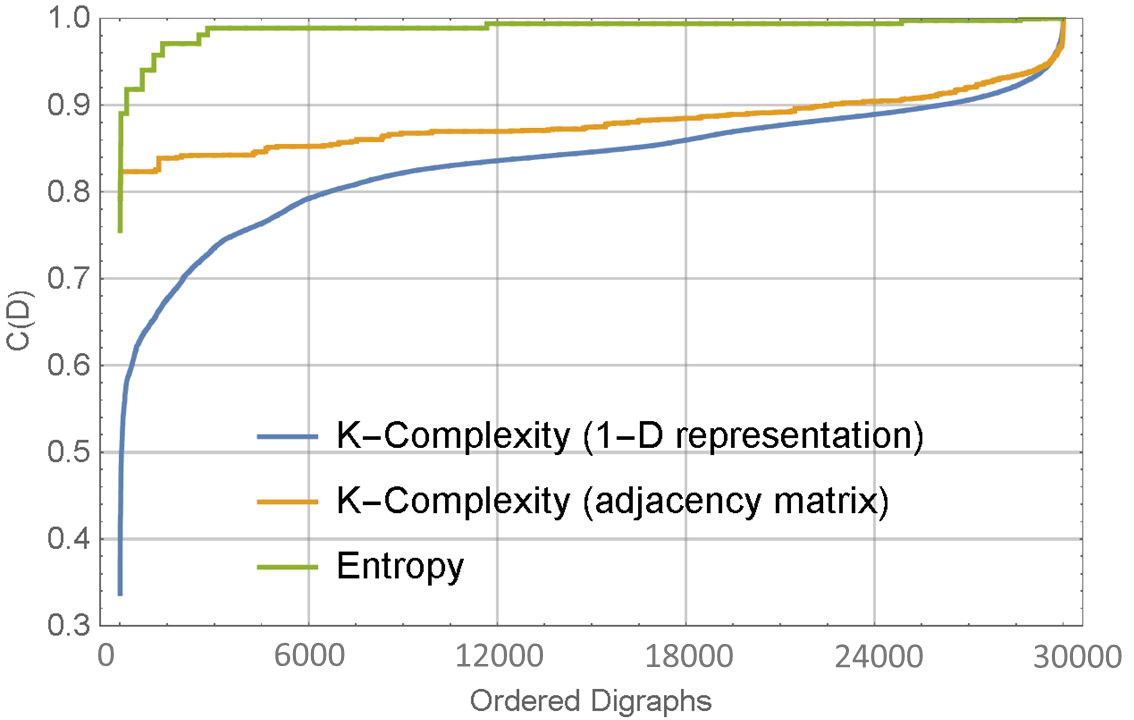
\includegraphics[width=\textwidth]{results_ordered_di_revisited_corrected}
		\caption{}
		\label{fig:results_ordered_di_revisited}
	\end{subfigure}
	%\\	
	\hfill
	%\hspace{0.5mm}
	\begin{subfigure}[b]{0.65\textwidth}
		\centering
		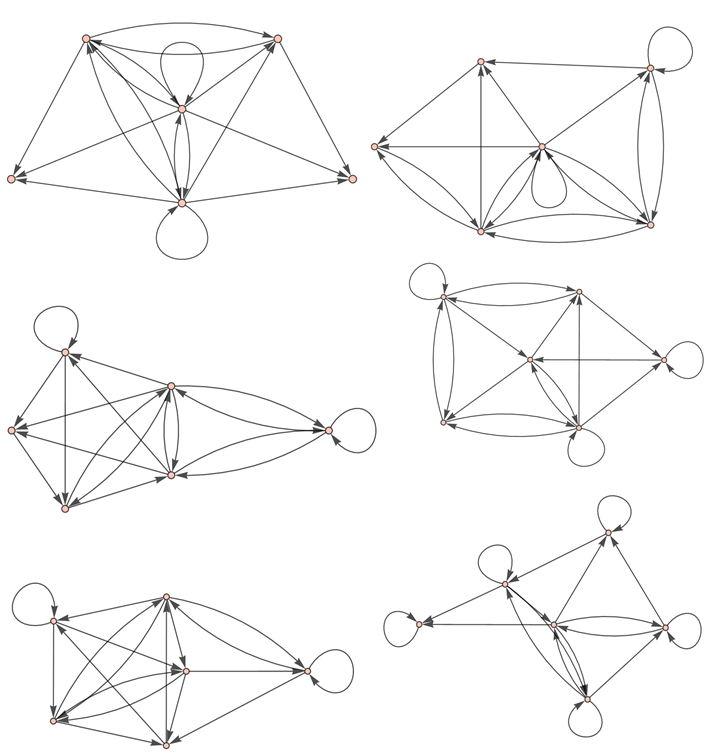
\includegraphics[width=\textwidth]{digraphs_increasig_complexity_revisited}
		\caption{}
		\label{fig:digraphs_increasig_complexity_revisited}
	\end{subfigure}
	\caption[Complexity measurements for random digraphs considering its isomorphisms.]{(a) Complexity measurements for random digraphs. The results were ordered by increasing complexity value. The number of random digraphs generated was $30,000$ and all they had $6$ nodes and vertex in-degree $3$. The number of random permutations in the labels of the nodes used at each iteration to generate the isomorphisms was $1000$, but only which resulted not repeated were considered. For purposes of comparison, the results obtained with each method were normalized with respect to the maximum value. (b) Some directed graphs plotted by increasing complexity value. The complexity increases from left to right and from up to down. The order was obtained from the complexity measurements from the K-complexity method using a 1-D representation. The digraphs plotted were chosen from regular intervals of complexity, such that the digraph at the upper left corner is the less complex and the digraph at the lower right corner is the most complex digraph generated in the experiment.}
	\label{fig:digraphs_increasig_complexity_results_revisited}
\end{figure}

The result of this experiment is shown in Fig. \ref{fig:digraphs_increasig_complexity_results_revisited} and the code used can be seen in the Appendix Section \ref{codes_wolfram} (Fig. \ref{fig:iso_D_k_cte_code}). As can be seen in Fig. \ref{fig:results_ordered_di_revisited} the complexity measurements showed the same behavior as in Fig. \ref{fig:results_ordered_di}. This is normal since the digraphs generated had the same number of nodes and the same vertex in-degree. Nevertheless, in Fig. \ref{fig:digraphs_increasig_complexity_revisited} it is possible to note a slightly different result. This time it is easier and clearer to visualize from the drawn digraphs, that the less complex digraph is indeed less complex than the more complex digraph. The less complex digraph seems to be more symmetrical while the more complex digraph is totally asymmetrical. Thus, in this experiment, we have reconciled our intuition of how a complex digraph should look like and how a digraph which is not so complex should look like.\\

The results of this experiment are important since any complexity measurement must agree with our intuition about what should be considered complex otherwise the method would be useless. We saw in Section \ref{complex_seqs_section} how the measurements of complexity obtained with several methods agree with our intuition about the complexity of binary sequences, however, now we have seen that they also agree with our intuition about the complexity of digraphs. This result is what we needed to be sure the methods we have been using give results which are correct, i.e., they correctly measure the complexity of digraphs. This approach to verify our measurements was not needed previously (sections \ref{comp_graphs_section} and \ref{comp_incr_vert_in_section}) since there we had a parameter which controlled the complexity of the networks, so we only had to ensure the agreement between the complexity measurements and this parameter. Nevertheless, our findings about the complexity of isomorphisms would not have been possible without this experiment since, until the experiment for the complexity from the uniform digraph distribution (section \ref{uni_di_dist_section}), the results seemed to be consistent.

\section{The Complexity of a Set Boolean Functions}
As indicated before, a Random Boolean Network is defined by its topology and its updating functions. In the last section, we devoted to learned how the complexity of the topology can be measured. Now, in this section, we will try to establish a systematic way to measure the complexity of the updating functions.\\

As it can be remembered, in a Boolean Network of $N$ nodes, we assign to each node a logic function of $k$ inputs. We denote this set of Boolean functions belonging to a Boolean Network as $f= \{ f_{1},f_{2},...,f_{N} \}$.\\

Here, we propose the following method to measure the complexity of a set of Boolean functions. First, it must be remembered that the behavior of each Boolean function $f_{i}$ can be described by its truth table. Hence, the behavior of a set of Boolean functions can be described by a set of truth tables. From this set of Boolean functions, we can build a unique truth table as a representation of all of them. As this unique truth table contains all the information about the set of Boolean functions, a measurement of its complexity equals to measure the complexity of the set of Boolean functions. Finally, this unique truth table is a matrix which can be used as a lossless representation of the set of Boolean functions.\\

For instance, in Section \ref{dynamics_ex_rbn}, we saw an example of Random Boolean Network with the assigned logic functions we reproduce again in Table \ref{tab:example_truth_table2}. From this truth table, we can build the representation shown in Fig. \ref{fig:matrix_truth_table}. This representation is a matrix with dimensions $2^{k} \times N$, thus we can apply to it the same methods we have used to measure the complexity of adjacency matrices in sections \ref{comp_graphs_section} and \ref{complex_di_section}.\\

\begin{table}[h]
\centering
\begin{tabular}{ |c||c|c|c|c| } 
 \hline
 $\sigma_{1}$	$\sigma_{2}$ & $f_{Node 1}$ & $f_{Node 2}$ & $f_{Node 3}$ & $f_{Node 4}$ \\ 
 \hline
 \hline
 0	0 & 1& 1& 0& 1\\ 
 \hline
 0	1 & 1& 1& 1& 1\\
 \hline
 1	0 & 0& 0& 1& 0\\
 \hline
 1	1 & 0& 1& 0& 0\\
 \hline
\end{tabular}
 \caption{Truth table with the set of Boolean functions assigned to a Boolean Network of $4$ nodes and parameter $k=2$ used to write the matrix representation of the set of updating functions.}
 \label{tab:example_truth_table2}
\end{table}

\begin{figure}[h]
\centering
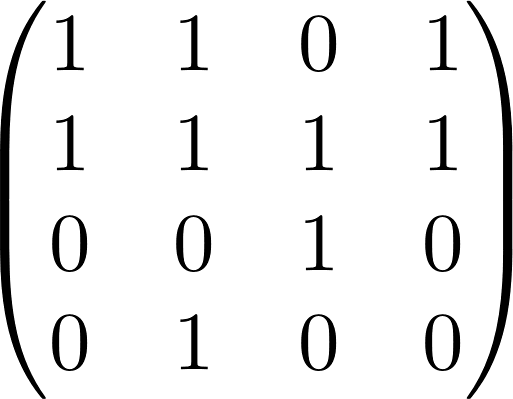
\includegraphics[scale=0.18]{matrix_truth_table}
\caption[Matrix representation of a set of Boolean functions.]{Matrix representation of the truth table shown in \ref{tab:example_truth_table2}.}
\label{fig:matrix_truth_table}
\end{figure}

In the next sections, two experiments will be performed to check out if this representation of the set of Boolean functions of a Boolean Network delivers results which makes sense when measuring its complexity.

\subsection{The Complexity from Sets of Random Boolean Functions with Increasing Number of Inputs}
This first experiment is inspired by the experiments of sections \ref{Watts-Strogatz_section}, \ref{barabasi_experiment_text} and \ref{comp_incr_vert_in_section}. In those experiments, we had a parameter which controlled the complexity of the random networks generated at each iteration. In this way, we were able to confirm that our measurements of complexity had the behavior expected according to the value of this parameter.\\

Similarly, in this experiment, at each iteration, a set of $N$ random Boolean functions with $k$ inputs will be generated. The logic functions will be randomly chosen from the uniform probability distribution of the $2^{2^{k}}$ possible Boolean functions with $k$ inputs. Thus, the number of possible sets of random functions is given by $2^{N \times 2^{k}}$ as was shown in Eq. \ref{number_rbn}.\\

Since in any Random Boolean Network model, the number of nodes must remain fixed throughout the dynamics. In this experiment, the parameter $N$ also will remain fixed and the complexity of the randomly generated sets of boolean functions will be controlled by the parameter $k$.\\

At each iteration, the matrix representation for each set of logic functions randomly generated will be built and used to measure its complexity. As was usual in the previous sections, the K-complexity will be directly measured from the matrix representation\footnote{The method we have been using was originally created to measure the complexity of adjacency matrices, i.e., square matrices, nevertheless thanks to the BDM Method, it can be also used to measure the complexity of non-square matrices.}, but also a 1-D lossless representation will be created from this matrix to measure the entropy and the 1-dimensional K-complexity. Moreover, as was did in sections \ref{Watts-Strogatz_section}, \ref{barabasi_experiment_text} and \ref{comp_incr_vert_in_section}, the fluctuations in the results with a given value of $k$ will be reduced by means of a trimmed mean which will be made by generating a given number of sets with the same parameter value, for later compute the quartiles of the results and finally compute the mean value by considering only the second and third quartiles. The result of this procedure will be considered the complexity value we are looking for. At the end of the iteration, the parameter $k$ will be increased and the algorithm will be repeated.\\

As the value of the parameter $k$ increases, we expect that the complexity of the set of Boolean functions will also increase since the information needed to reproduce the behavior of a Boolean function with larger $k$ value is greater than for a shorter $k$.\\

\begin{figure}
\centering
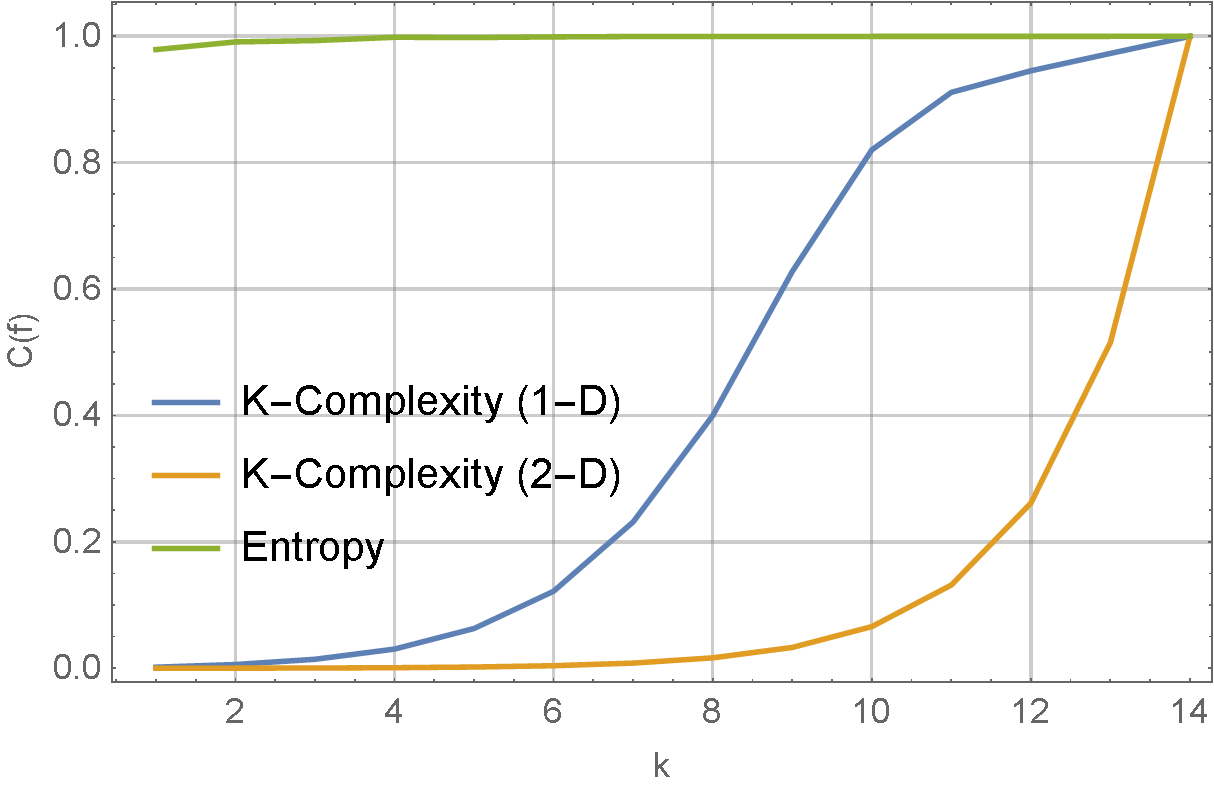
\includegraphics[width=\textwidth]{results_boolfuns_aum_k}
\caption[Complexity measurements using three different methods of random sets of Boolean functions.]{Complexity measurements using three different methods of random sets of Boolean functions obtained from a uniform distribution versus the parameter $k$ (the number of inputs). The sets generated had $10$ Boolean functions each one ($N=10$) and the parameter $k$ was vary from $1$ to $14$. The number of sets of random logic functions generated with the same $k$ value was $10$ from which the trimmed mean described before was done. For purposes of comparison, the results obtained with each method were normalized with respect to the maximum value.}
\label{fig:results_boolfuns_aum_k}
\end{figure}

The result of this experiment is shown in Fig. \ref{fig:results_boolfuns_aum_k}. The performance of the entropy method was awful, showing almost a constant behavior. On the other hand, the results with the K-complexity showed that the complexity increased when the parameter $k$ increased just as was expected. Nevertheless, the behavior of the Kolmogorov complexity differed depending on which representation was used. The results from the 2-D representation (the matrix representation) seemed to be almost constant from $k=1$ to $k=8$. Meanwhile, the results from the 1-D representation showed a gradual increase in all the range experimented. From these observations, we could be tempted to conclude that the 1-D representation method is better to measure the complexity of a set of Boolean functions. However, the range used is limited and does not allow to infer the behavior for a larger $k$ value, especially the behavior of the 1-D representation. Though, since the complexity should continue increasing it is almost sure that the 1-D representation will continue to be the best method for larger $k$ values.\\

The code used to generate sets of random Boolean functions and measure its complexity is shown in the Appendix Section \ref{codes_wolfram} (Fig. \ref{fig:set_bool_fun_k_inc_code}). Maybe the most interesting part of the code is the generation of random Boolean functions. One possible approach could have been to generate a matrix with dimensions $2^{k} \times N$ and initialize it with zeros. Then, given a parameter $p$, we could have changed the $0's$ by $1's$ on each column of the matrix (a column corresponds to a logic function). This procedure would be ideal if we were interested in the generalization of the original Kauffman model for a Random Boolean Network discussed in Section \ref{functions}. However, we are interested only in the original model proposed by Kauffman where for each node a Boolean function is randomly chosen within all the universe of possible functions with $k$ inputs, and where all the functions have the same probability to be chosen, i.e., the probability distribution is uniform. This random choice is easily implemented in Mathematica by means of the Built-in function \textit{BooleanFunction} which immediately allows accessing to all the $2^{2^{k}}$ possible Boolean functions with $k$ inputs. Then, the Boolean function chosen is represented as a combination of one of the universal Boolean functions defined in \ref{Universal_Boolean_Functions} by means of the built-in function \textit{BooleanConvert} and finally, the truth table is obtained by means of the built-in function \textit{Boole}. The truth tables are joined as described before, and in this way, the matrix representation is built. 


\subsection{The Complexity from Sets of Random Boolean Functions with Fixed Number of Inputs}
As happened before, the experiment with increasing parameter $k$ is not so interesting since in the CRBN model the parameter $k$ also remains fixed throughout the dynamics. Therefore, it desirable to perform an experiment where both parameter $N$ and $k$ could remain fixed. However, if these parameters are fixed, there will be no way to control the complexity of the sets of Boolean functions generated. This is the same problem we faced in sections \ref{uni_di_dist_section} and \ref{uni_di_dist_section_with_iso}. Thereby, the same approach used in those sections will be used to measure the complexity of sets of random logic functions.\\

The sets of random Boolean functions will be generated as in the last section, but this time with both parameters $k$ and $N$ fixed. For each set, the matrix representation will be built and from it, the complexity will be measured by means of the three methods we used in the former experiments. From the sections \ref{uni_di_dist_section} and \ref{uni_di_dist_section_with_iso} we learned that the complexity of an object depends on the isomorphic representation used. Thus, it will be necessary to measure again the complexity using different isomorphic representations and use the minimum value obtained as the true value of the complexity. An isomorphic representation of our matrix representation is easily obtained by permuting its rows. This permutation corresponds to a reorder on the input states \footnote{An alternative would be to consider the permutations on the columns, which corresponds to a reorder on the labels of the functions, i.e., a reassignment of the functions to the nodes. Nonetheless, if we were studying the dynamics of an RBN, this type of permutations would give a Boolean Network with a completely brand-new dynamics and thus the complexity measurements would correspond to different objects. Hence, even though we are not considering the dynamics of a Boolean function, this type of permutations will not be considered. }. For instance, the truth table in Table \ref{tab:example_truth_table2} presented the input states in a \textit{canonical order}: $\{ 00,01,10,11 \}$. Nevertheless, instead, we could have used the order $\{ 11,10,01,00 \}$ or any other, i.e., any other isomorphic representation. The number of possible permutations of the rows in our matrix representation with dimensions $2^{k} \times N$ is $2^{k} !$. Therefore, it could be computationally expensive to try all the possible permutations every time a set of random Boolean functions is generated. Thus, in order to measure its complexity, just a given number of permutations chosen randomly (with a uniform probability distribution) will be considered each time a set of random Boolean functions is generated.\\

Once the complexities of the isomorphic representations are measured, the minimum value obtained will be considered to be the complexity of the original matrix representation, i.e., the complexity of the set of Boolean functions. This procedure will be repeated a given number of times and the results will be ordered from the less to the greater complexity value. As happened in sections \ref{uni_di_dist_section} and \ref{uni_di_dist_section_with_iso}, we need a method to check out if the measurements of complexity we are getting make sense. In those sections, we relied upon a visual approach by drawing the digraphs to confirm that the extreme cases show a clear difference in complexity. In this experiment, as visual confirmation of the results, the matrix representation of every random set of Boolean functions will be plotted. To do so, we will take advantage of the fact that the matrix representation is built only by $0's$ and $1's$. In this way, the matrix elements will be represented in a grid where a square will be colored black if the corresponding matrix element is $1$, otherwise, if it is $0$, it will be colored white. This plotting is a visual representation of the set of Boolean functions since all the rules are contained within it.\\

It is expected that the less complex set of Boolean functions will be the set made up only by functions which deliver always a zero(one) for all the possible input states. Thus, its matrix representation is full of zeros(ones). On the other hand, the most complex set of Boolean functions must be a set where there is no apparent order in the distribution of $0's$ and $1's$.\\

\begin{figure}
	\centering
	\begin{subfigure}[b]{0.65\textwidth}
		\centering
		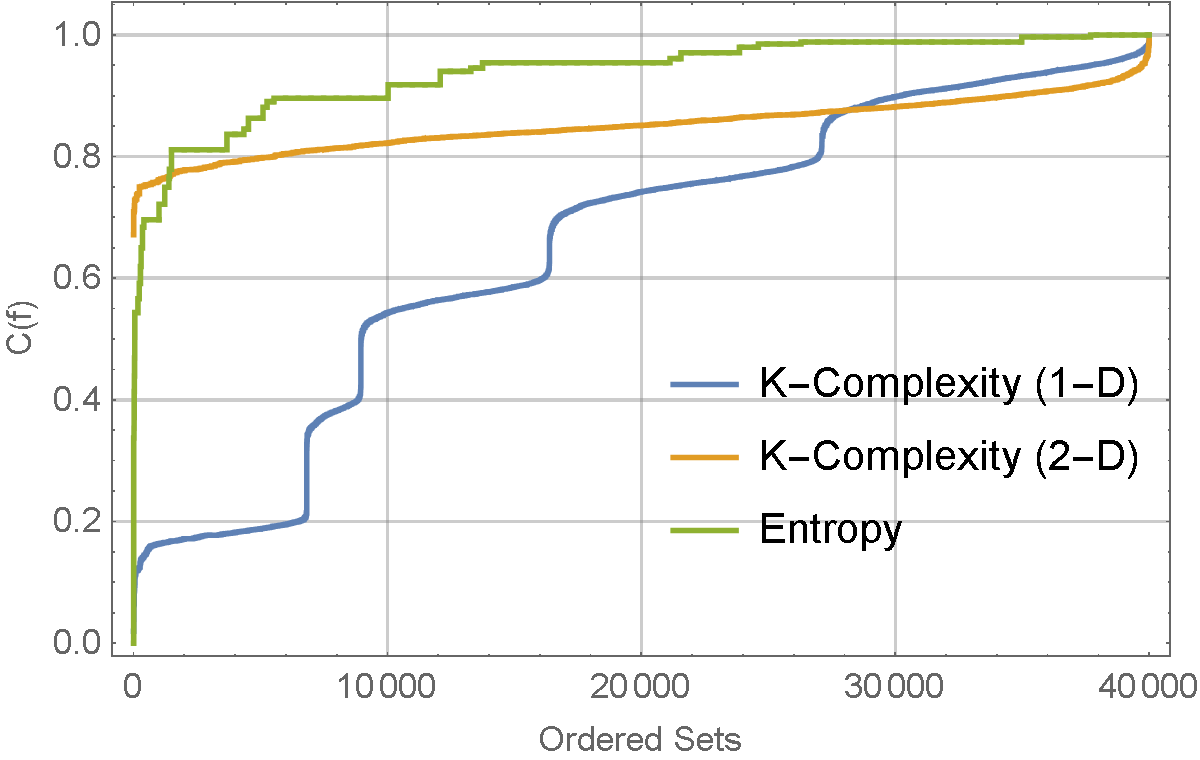
\includegraphics[width=\textwidth]{results_ordered_sets}
		\caption{}
		\label{fig:results_ordered_sets}
	\end{subfigure}
	%\\	
	\hfill
	%\hspace{0.5mm}
	\begin{subfigure}[b]{0.6\textwidth}
		\centering
		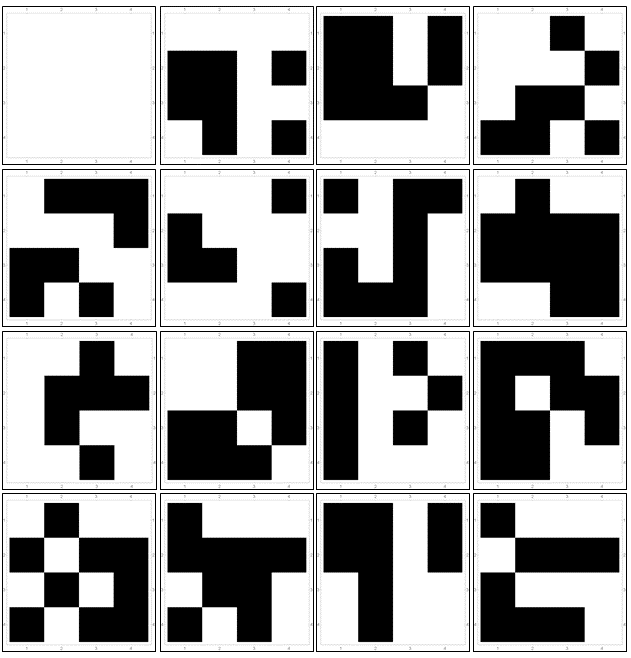
\includegraphics[width=\textwidth]{complexity_ordered_sets}
		\caption{}
		\label{fig:complexity_ordered_sets}
	\end{subfigure}
	\caption[Complexity measurements for sets of random Boolean functions sorted by increasing complexity value.]{(a) Complexity measurements for sets of random Boolean functions. The results were sorted by increasing complexity value. The number of random sets generated was $40,000$ and all they had $4$ functions ($N=4$) each one with $k=2$ inputs. At each iteration, the number of randomly generated permutations of the rows in the matrix representation was $16$, but only the permutations which resulted not repeated were considered. For purposes of comparison, the results obtained with each method were normalized with respect to the maximum value. (b) Some sets of Boolean functions plotted by increasing complexity value. The complexity increases from left to right and from up to down. The order was obtained from the complexity measurements from the K-complexity method using the 1-D representation. The sets of logic functions plotted were chosen from regular intervals of complexity, such that the set at the upper left corner is the less complex and the set at the lower right corner is the most complex set of Boolean functions generated in the experiment. Each set is represented by a square whose columns represent the logic functions and its rows represent the possible input states.}
	\label{fig:sets_bool_results}
\end{figure}

The result of this experiment is shown in Fig. \ref{fig:sets_bool_results}. As can be seen in Fig. \ref{fig:results_ordered_sets}, it seems that the three methods are able to measure a gradual increase in the complexity of the sets of Boolean functions. The results of the K-complexity with a 1-D representation showed a stairway like behavior meanwhile the 2-D representation showed a smoother curve. Surprisingly, the entropy method this time did not show a slope almost equal to zero as it did in the former experiments. Nonetheless, the range of complexity values shown by the entropy and the K-complexity with the 2-D representation was very limited when compared with the range of complexity values computed with the method of K-complexity and the 1-D representation, which means that this last method was able to capture with more detail the changes in complexity on the sets of Boolean functions. Thus, this method proved again to be the best, this time by measuring the complexity of sets of Boolean functions.\\

Meanwhile, the results in Fig. \ref{fig:complexity_ordered_sets} showed as expected, that the less complex set of Boolean functions is the set whose matrix representation is full of zeros. In general, among two sets of Boolean functions, it is hard to say which one is more complex just from the visual representation. However, the correct prediction of the less complex set of Boolean functions gives confidence in that the method to compute the complexity is working as it should so we do not have to depend on a visual representation anymore.\\

The code used to generate sets of random Boolean functions and measure its complexity is shown in the Appendix Section \ref{codes_wolfram} (Fig. \ref{fig:set_bool_fun_code}). It is like the code shown in Fig. \ref{fig:set_bool_fun_k_inc_code}, but this time the parameter $k$ remains fixed and the complexity is measured with the help of the isomorphic representations as was described before.

\section{The Complexity of Boolean Networks}
In the last sections, we already have studied the complexity of the components of Boolean Networks, i.e., the topology and the updating functions, though we have studied them separately. Nonetheless, measuring the complexity of the components of a Boolean Network separately and then simply adding them up should not be equal to simply measuring the complexity of a Boolean Network when it acts as an ensemble. The interaction between the topology and the updating functions is so intricate that a measurement of these components separately must be a poor approximation to the real complexity of the system. Of course, it is expected that a topology which is simple will produce a Boolean Network which also is simple and the same should happen for the Boolean functions, indeed we are going to investigate further this hypothesis lately, but the question of how to measure the complexity of a Boolean Network still exists.\\

We will try to answer this question by appealing to Definition \ref{Alternative_Definition} of a Boolean Network. In this definition a Boolean Network is seen as a logic function which maps $f: \{0,1 \}^{N} \rightarrow \{0,1 \}^{N}$ and where $N$ is the number of nodes. Therefore, if we wish to measure the complexity of a Boolean Network, we must measure the complexity of its behavior when acting as a function, i.e., we must measure the complexity of the mapping produced by it. The mapping produced by the Boolean Network contains all the information about its topology and its updating functions, moreover it contains the information of these constituents when acting together, so its complexity must correspond to the complexity of the Boolean Network.\\

\subsection{A Lossless Representation for Boolean Networks}
Following the previous arguments, in this section, a lossless representation of the mapping produced by a Boolean Network is presented. The method will be introduced through an example.\\

In Table \ref{tab:example} and Fig. \ref{fig:di_example} were shown respectively, the updating functions and the topology of a Boolean Network. Meanwhile, in Fig. \ref{fig:rbn_example} was shown the state-space corresponding to this Boolean Network. This state-space represents the dynamics of the system, i.e., the mapping of the Boolean Network since it says to what state the system should move given any input state. From this state space, the Table \ref{tab:mapping_ex} can be built. This table represents the mapping made by the Boolean Network.\\

\begin{table}[h]
\centering
\begin{tabular}{ |c|c| } 
 \hline
 Input State & Output State\\ 
 \hline
 \hline
 0000	& 1101\\ 
 \hline
 0001	& 1111\\
 \hline
 0010	& 1101\\
 \hline
 0011	& 1111\\
 \hline
 0100	& 1101\\
 \hline
 0101	& 1111\\
 \hline
 0110	& 1101\\
 \hline
 0111	& 1111\\
 \hline
 1000	& 0010\\
 \hline
 1001	& 0100\\
 \hline
 1010	& 0010\\
 \hline
 1011	& 0100\\
 \hline
 1100	& 0010\\
 \hline
 1101	& 0100\\
 \hline
 1110	& 0010\\
 \hline
 1111	& 0100\\
 \hline
\end{tabular}
 \caption[The mapping produced by a Boolean Network.]{The mapping produced by the Boolean Network presented in Table \ref{tab:example} and Figs. \ref{fig:di_example} and \ref{fig:rbn_example}. The input states were placed in canonical order by considering them as binary numbers.}
 \label{tab:mapping_ex}
\end{table}

A lossless representation of the mapping produced by the Boolean Network can be built just by putting each output state one after the other in the same order shown in Table \ref{tab:mapping_ex}:

\begin{quote}
\centering
S=1101111111011111110111111101111100100100001001000010010000100100
\end{quote}


This binary sequence is a lossless representation of the mapping produced by the system and its complexity should correspond as was argued before to the complexity of the Boolean Network \footnote{It is not necessary to consider the input states in the representation of the Boolean network because its effect only would be to add a constant to the complexity of the Boolean Networks.}. Furthermore, since it is a binary sequence, we can measure its complexity by using the same methods of Section \ref{complex_seqs_section}.\\

Now that we have a way to represent a Boolean Network as a simple binary sequence and thus a way to measure its complexity, some experiments will be performed in the following sections concerning the complexity of Random Boolean Networks.

\subsection{The Correlation Between the Complexity of Random Boolean Networks and The Complexity of Its Topology}
\label{correlation_com_topology}
If we have a given set of Boolean functions and randomly choose a topology for this set, in order to create an RBN, every different topology chosen will make the RBN to have a different complexity value. It is expected that a topology which is simple will render a Boolean Network which also is simple and in the same way, a topology which is complex should produce a Boolean Network which is complex as well. In other words, there should exist a positive correlation between the complexity of a Boolean Network and the complexity of its topology. In this section, this ansatz will be tried to be verified. To do so, the next procedure is used.\\

Firstly, a random topology is chosen following the classical Random Boolean Network model with a given number of nodes and vertex in-degree (see Section \ref{topology_section}). Then, a given number of random sets of updating functions is chosen following the classical Kauffman model as well (see Section \ref{functions}). Thereupon, these sets of Boolean functions are assigned to the topology generated before, which means we are creating RBNs with the same topology, but with different updating functions. The dynamics of the RBN is generated by introducing to it all the possible input states and from this, the lossless representation discussed before is created for each RBN and its complexity is measured by using the K-complexity implementation, as was used in Section \ref{complex_seqs_section} to measure the complexity of random binary sequences. From the complexities obtained for the RBNs, the quartiles of this set of results were calculated, and by only considering the second and third quartiles, the mean complexity was computed, i.e., we computed a trimmed mean. Therefore, we were interested in knowing the mean complexity of RBNs which share the same topology and for which only the updating functions were varied among them.\\

Afterward, the complexity of the topology is measured by considering some of its different isomorphic representations. In Section \ref{comp_iso_net_section}, the true complexity value of the topology was considered to be the lower value obtained with these isomorphic representations. Nevertheless, this time we will consider the mean complexity of the topology from its isomorphic representations and not the minimum value as before. The reason is because we will be measuring the mean complexity of Random Boolean Networks with this same topology, therefore it is desirable to measure also the mean complexity of the topology since it could happen for example, that we assign the same set of updating functions to the topology, but with the functions sorted in different order. That would correspond to Boolean Networks which share the same set of updating functions, but with isomorphic topologies. Therefore, it is better to consider the mean of the complexity of the isomorphic topologies and not just one value (the minimum value).\\

Thereupon, a new topology is randomly chosen, again with the same parameters, and in the same way, new sets of updating functions are randomly generated to create RBNs and measure its mean complexity together with the mean complexity of its topology and so on.\\

%Once we have all the results, they are plotted, and a linear model is fitted to them. Thereupon, the correlation between the two complexities is tested by means of the built-in function \textit{IndependenceTest} of Mathematica. This function automatically chooses the best test that applies to the given data and returns a coefficient value which allows to confirm or reject the dependence between the variables.\\
Once we have all the results, they are plotted, and the correlation between the two complexities is evaluated by computing the \textit{Pearson correlation coefficient} to test a possible linear correlation. Additionally, a linear model is fitted to the data. However, since we do not know whether the possible correlation between the variables is linear or not, also the \textit{Spearman's rank correlation coefficient} is computed to evaluate how well the relationship between the two complexities is described by a monotonic function.\\

Due to the high computational cost to generate Random Boolean Networks and compute its complexity, this experiment was performed with small topologies, specifically, a topology with five nodes and other with seven nodes were considered. Another reason to consider small topologies is the huge number of possible RBNs with larger topologies. As was said in Section \ref{Counting_RBN_section}, the number of possible Random Boolean Networks increases so fast with the parameters $N$ and $k$. Hence, it is hard to perform statistics in this ensemble since larger topologies would make even harder to get enough data to statistically be able to conclude something. For these reasons, we will focus on RBNs with just a few nodes.\\

%\begin{figure}
%\centering
%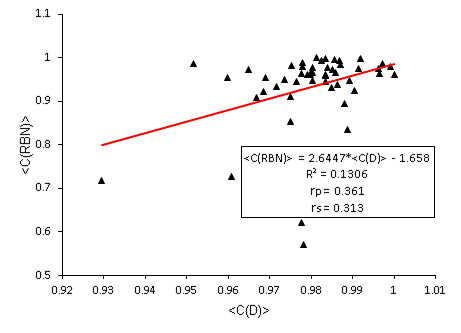
\includegraphics[width=\textwidth]{results_rbn_graf_cte1}
%\caption[Correlation between the complexity of Random Boolean Networks and its topology.]{The mean complexity of the topology versus the mean complexity value of Random Boolean Networks with this same topology. Both complexities were normalized with respect to its maximum value. All the topologies used had five nodes ($N=5$) and vertex in-degree $3$. The number of RBNs generated with the same topology at each iteration was $5000$ and the number of random permutations generated to measure the complexity of the topology was $300$, though only which resulted not repeated were considered. A linear model was fitted to the results. The model fitted has an intersection with the vertical axis at $-1.658$ and a slope of $2.6447$ with an $R^{2}$ coefficient of $0.13$. The best method to test the correlation between the complexities was found to be the Spearman's rank correlation coefficient which value resulted to be $\rho =0.313$.}
%\label{fig:results_rbn_graf_cte1}
%\end{figure}



\begin{figure}
	\centering
	\begin{subfigure}[b]{0.64\textwidth}
		\centering
		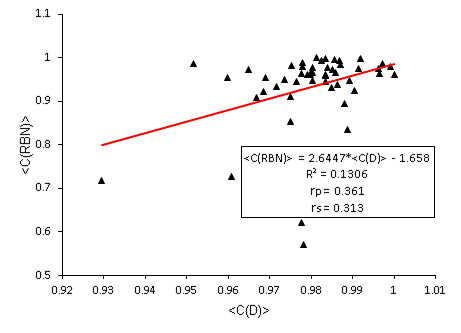
\includegraphics[width=\textwidth]{results_rbn_graf_cte1}
		\caption{}
		\label{fig:results_rbn_graf_cte1}
	\end{subfigure}
	%\\	
	%\hfill
	\hspace{0.1mm}
	\begin{subfigure}[b]{0.64\textwidth}
		\centering
		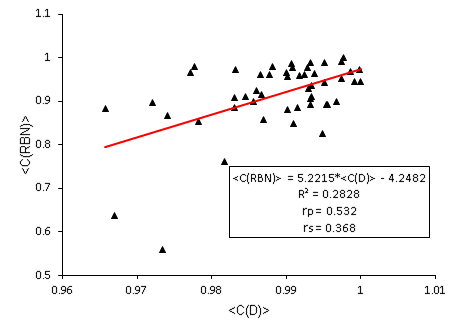
\includegraphics[width=\textwidth]{results_rbn_graf_cte2}
		\caption{}
		\label{fig:results_rbn_graf_cte2}
	\end{subfigure}
	\caption[Correlation between the complexity of Random Boolean Networks and its topology.]{The mean complexity of the topology versus the mean complexity of Random Boolean Networks with this same topology. Both mean complexities were normalized with respect to its maximum value.  A linear model was fitted to the results and the correlation between the variables was studied. (a) All the topologies used had five nodes ($N=5$) and vertex in-degree $3$. The number of RBNs generated with the same topology at each iteration was $5000$ and the number of random permutations generated to measure the mean complexity of the topology was $300$, though only which resulted not repeated were considered. The model fitted has an intersection with the vertical axis at $-1.658$ and a slope of $2.6447$ with an $R^{2}$ coefficient of $0.13$. The Pearson correlation coefficient resulted to be $r_{P} =0.361$, while the Spearman's rank correlation coefficient resulted to be $r_{S} =0.313$. (b) All the topologies used had five nodes ($N=7$) and vertex in-degree $4$. The number of RBNs generated with the same topology at each iteration was $2000$ and the number of random permutations generated to measure the mean complexity of the topology was $5000$, though only which resulted not repeated were considered. The linear model fitted has an intersection with the vertical axis at $-4.2482$ and a slope of $5.2215$ with an $R^{2}$ coefficient of $0.282$. The Pearson correlation coefficient resulted to be $r_{P} =0.532$, while the Spearman's rank correlation coefficient resulted to be $r_{S} =0.368$.}
	\label{fig:results_rbn_graf_cte}
\end{figure}

The results of two experiments performed with different parameters $N$ and $k$ are shown in Fig. \ref{fig:results_rbn_graf_cte}. As can be seen in both experiments, the data showed a linear relationship between the mean complexity of the RBNs and the mean complexity of the topologies used. The Pearson correlation coefficient computed for the complexities in Fig. \ref{fig:results_rbn_graf_cte1} was $r_{P} =0.361$, while the Spearman's rank correlation coefficient computed was $r_{S} =0.313$. These values indicated that there exists a correlation between these complexities as was expected. Furthermore, the linear correlation is slightly stronger than a correlation described by a monotonic function. Moreover, the coefficients are positive which means that a greater mean complexity value for the RBN corresponds to greater mean complexity for the topology used. The same happened for the complexities showed in Fig. \ref{fig:results_rbn_graf_cte2} which had a Pearson correlation coefficient of $r_{P} =0.532$ and a Spearman's rank correlation coefficient of $r_{S} =0.368$. These values were closer to $1$ than they were in the first experiment which means that both correlations were stronger. In fact, the Pearson correlation coefficient is greater than $0.5$ so we can consider that both complexities showed a strong linear relationship.\\

According to the previous results, our initial hypothesis was correct, i.e., a simple RBN indicates a simple topology and a complex RBN indicates a complex topology. Furthermore, the correlation seems to be linear. Nonetheless, it seems there exist cases, where this hypothesis is not fulfilled. This can be explained by the fact that the complexity of a Boolean Network also is determined by the updating functions which were chosen and not only by the topology used. To see this, just imagine we assign to a topology very complex the updating functions whose matrix representation is full of zeros, then no matter which input state we evaluate, since the state of the network will always be the same. Thus, this type of updating functions spoils the complexity of the network. This explains why the the Pearson correlation coefficient and the Spearman's rank correlation coefficients found in these experiments are positive but not equal to $1$. Unfortunately, this experiment is not enough to say that our hypothesis has been demonstrated empirically for any Boolean Network. To do so, it it would be necessary to perform more experiments with topologies of distinct sizes. All we can say is that our hypothesis of correlation was correct for Random Boolean Networks with small topologies given an ensemble with a sufficiently large number of Boolean Networks.\\

The code used in this experiment can be found in the Appendix Section \ref{codes_wolfram} (Fig. \ref{fig:rbn_vs_graph_complexity}). Almost all the code has been recycled from previous experiments. The only difference is the section which allows testing the output states of the Boolean Network given all the possible input states, i.e., the section which gives the dynamics of the network.

\subsection{The Width of the Distribution of Complexities for Random Boolean Networks}
In the last section, the complexities of Random Boolean Networks which shared the same topology were calculated, and from them, the mean complexity of these RBN was computed. Now, we will study the standard deviation in the complexities from which the mean is calculated, i.e., we will examine the behavior of the width in the distribution of complexities of RBNs with the same topology. Specifically, we are interested in figuring out if this width stays constant or almost constant when the number of nodes is fixed.\\

We will use the results of the two experiments performed in the last section. From them, we will compute the standard deviation in the complexities of RBNs which share the same topology and where all the topologies have the same number of nodes and vertex in-degree.\\

\begin{figure}
	\centering
	\begin{subfigure}[b]{0.7\textwidth}
		\centering
		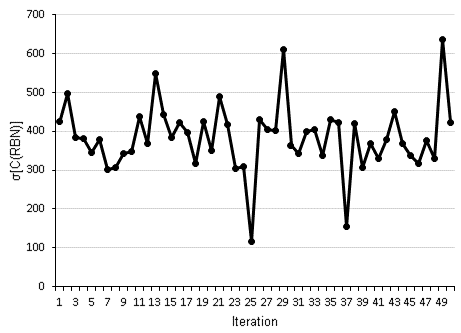
\includegraphics[width=\textwidth]{results_standard_node_cte1}
		\caption{}
		\label{fig:results_standard_node_cte1}
	\end{subfigure}
	%\\	
	\hfill
	%\hspace{0.5mm}
	\begin{subfigure}[b]{0.7\textwidth}
		\centering
		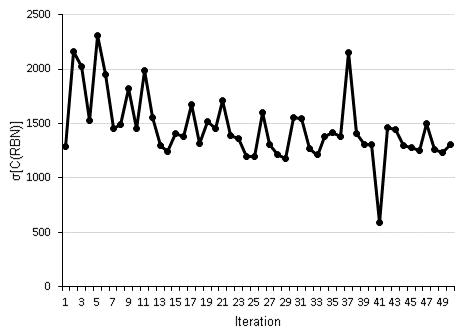
\includegraphics[width=\textwidth]{results_standard_node_cte2}
		\caption{}
		\label{fig:results_standard_node_cte2}
	\end{subfigure}
	\caption[The standard deviation in the complexities of Random Boolean Networks with fixed number of nodes.]{The standard deviation in the complexities of Random Boolean Networks with fixed number of nodes. (a)RBNs whose topology has $5$ nodes and vertex in-degree $3$. (b)RBNs whose topology has $7$ nodes and vertex in-degree $4$.}
	\label{fig:results_standard_node_cte}
\end{figure}


The results of these two experiments are shown in Fig. \ref{fig:results_standard_node_cte}. Both experiments confirmed that when the number of nodes is maintained fixed, the width of the distribution of complexities of RBNs with the same topology fluctuates randomly, though it seems to be bounded from above and from below. Given this behavior, it is expected that as the number of nodes increases, the standard deviation also will increase, i.e., the bounds of the fluctuations in the standard deviation will be moved according to the number of nodes.\\

Therefore, to analyze the behavior of the width in the complexity distribution of Random Boolean Networks against the number of nodes of the topology a modified version of the experiments shown in Fig. \ref{fig:results_rbn_graf_cte} was implemented. In this version, instead of fixing the number of nodes, at every certain number of iterations, this parameter is increased. The number of nodes starts in $2$ and the vertex in-degree remains fixed all the time. Thereupon, a random topology and a random set of updating functions are generated and with them, the dynamics of the network is generated. After, the complexity of the Random Boolean Network is measured as before. Since this occasion we are only interested in the distribution of complexities of the RBNs, it is not necessary to measure the complexity of the topology and the updating functions. Once we have generated and measured the complexity of a certain number of RBNs the number of nodes of the topologies (and the number of updating functions in the set of updating functions) is increased and the procedure is repeated. The standard deviation is computed for the complexities of each set of Random Boolean Networks which have the same number of nodes.\\

\begin{figure}
\centering
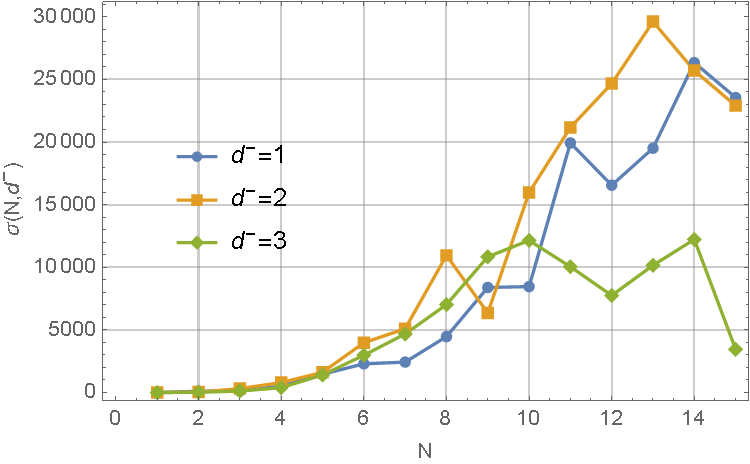
\includegraphics[width=\textwidth]{final_sigmas_igual_rbn}
\caption[The width of the distribution of complexities of Random Boolean Networks versus the number of nodes of the topologies.]{The width of the distribution of complexities of Random Boolean Networks versus the number of nodes of the topologies used. The experiment was performed with three different vertex in-degrees: $d^{-}=1,2$ and $3$. The number of RBNs generated with the same number of nodes, i.e., the size of the ensembles considered, was $100$ for the three parameters. The number of nodes ranged from $2$ to $16$.}
\label{fig:final_sigmas_igual_rbn}
\end{figure}

%The standard deviation in the complexities of Random %Boolean Networks Versus The Number Of Nodes

The result of this experiment is shown in Fig. \ref{fig:final_sigmas_igual_rbn}. The experiment was implemented with the vertex in-degrees $1,2$ and $3$. In the beginning, the width of the distribution of complexities increased monotonically with the number of nodes, however, it started to fluctuate with larger topologies. These fluctuations could be attributed to the fact that the number of possible RBNs increases fast with the number of nodes, therefore when the number of nodes of the topology was increased, the number of RBNs studied was not enough to keep the increasing of the width. It can be expected that the width will continue increasing with the number of nodes in an unbounded way with a sufficiently large ensemble of Random Boolean Networks. This hypothesis is reinforced by comparing the results with different vertex in-degree values. For topologies with a small number of nodes, the width of the distribution of complexities increased equally and independent of the parameter $d^{-}$. The behavior started to depend on the value of the vertex in-degree used, only for larger topologies. Thus, by remembering that the number of possible Random Boolean Networks increases not only with the number of nodes but also with the parameter $d^{-}$ (Eq. \ref{number_rbn_final}), and since the size of the ensembles of Random Boolean Networks used was the same for the three values of $d^{-}$, it is expected that the fluctuations would be significantly more important for $d^{-}=3$ than for the other values since our finite sample is less representative in this case due to the larger number of possible RBNs which were not considered. By following the same reasoning, the fluctuations for $d^{-}=2$ would have to be more important than for $d^{-}=1$. The previous can be checked in Fig. \ref{fig:final_sigmas_igual_rbn}, as can be seen from the results, when the value $d^{-}=3$ was used, the increase in the width was stopped and started to fluctuate earlier than for the other values. Moreover, for $d^{-}=2$ the increase was stopped earlier than for $d^{-}=1$. Hence, as was mentioned before, we expect that by considering ensembles of Random Boolean Networks sufficiently large, the width of the distribution of complexities will continue increasing monotonically with the number of nodes and independently of the vertex in-degree of the topologies used, i.e., we can expect a monotonically increasing behavior as the one shown in Fig. \ref{fig:expected_sigmas}.\\

\begin{figure}
\centering
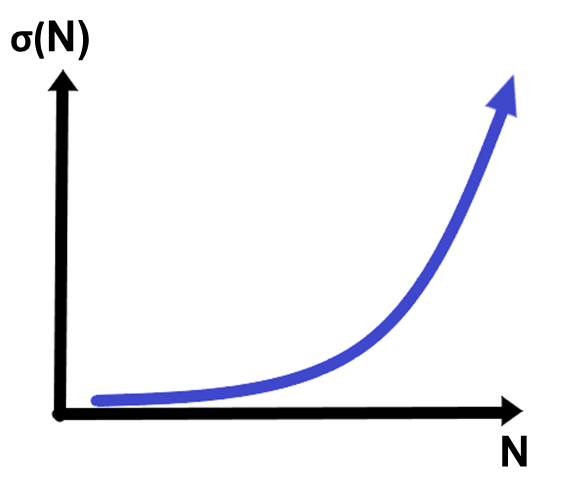
\includegraphics[scale=0.5]{expected_sigmas}
\caption[The expected behavior of the width of the distribution of complexities of Random Boolean Networks versus the number of nodes of the topologies.]{The expected behavior of the width of the distribution of complexities of Random Boolean Networks versus the number of nodes of the topologies used for ensembles sufficiently large. The value of $\sigma$ increases monotonically with the number of nodes and does not depend on the value of the parameter $d^{-}$, i.e., $\sigma = \sigma (N)$.}
\label{fig:expected_sigmas}
\end{figure}

This experiment can be performed with the code shown in Fig. \ref{fig:rbn_vs_graph_complexity} or Fig. \ref{fig:rbn_vs_func_complexity} (Appendix Section \ref{codes_wolfram}). The only change necessary is to increase the parameter $N$ every determined number of iterations at the beginning of the first iteration loop. For better performance, the parts which measure the complexities of the topology and the updating functions can be ignored. 

\subsection{The Correlation Between the Complexity of Random Boolean Networks and the Complexity of its Set of Updating Functions}
In the last sections, the correlation hypothesis between the mean complexity of the RBNs and the mean complexity of its topology was tested. Nonetheless, a Boolean Network is not defined by its topology but also by its updating functions. Hence, it is also expected that if the set of updating functions assigned to the network is simple, then the complexity of the Boolean Network also will be simple. This can be seen by testing the dependence of the variables as was did before.\\

The experiment is very similar to the one of Section \ref{correlation_com_topology}. However, this time a random set of updating functions was generated firstly. Then, some given number of topologies were randomly generated, and we assigned to all of them the same set of updating functions generated before. The complexity of the resulted Random Boolean Networks was measured and from the results, the mean complexity was computed by only considering the second and third quartiles of the data (trimmed mean). For the same reasons argued in Section \ref{correlation_com_topology}, the mean complexity of the set of updating functions was computed by considering its isomorphic representations and by discarding the first and fourth quartiles to compute the mean complexity (trimmed mean) instead of considering the minimum value of complexity. Thereupon, another set of updating functions was generated and the procedure was repeated.\\

Due to the same reasons for the experiment in Section \ref{correlation_com_topology}, this experiment was performed with topologies of only a few nodes. To be consistent, it was decided to perform again two experiments with the same parameters used before, i.e., the first experiment uses topologies with five nodes and vertex in-degree $3$ and the second experiment uses topologies with seven nodes and vertex in-degree $4$.\\

\begin{figure}
	\centering
	\begin{subfigure}[b]{0.64\textwidth}
		\centering
		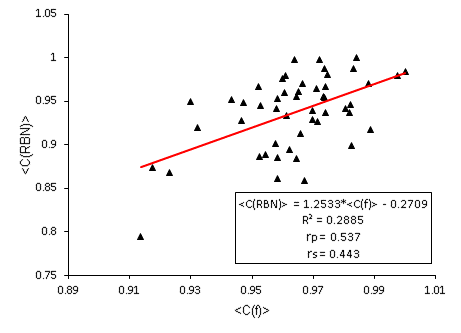
\includegraphics[width=\textwidth]{results_rbn_fun_cte1}
		\caption{}
		\label{fig:results_rbn_fun_cte1}
	\end{subfigure}
	%\\	
	\hfill
	%\hspace{0.5mm}
	\begin{subfigure}[b]{0.64\textwidth}
		\centering
		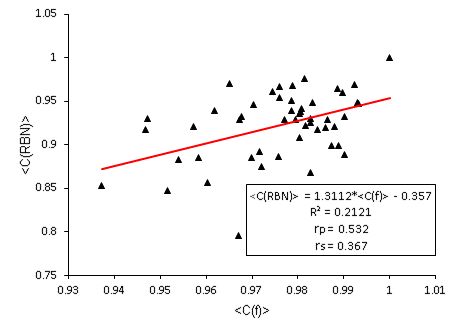
\includegraphics[width=\textwidth]{results_rbn_fun_cte2}
		\caption{}
		\label{fig:results_rbn_fun_cte2}
	\end{subfigure}
	\caption[Correlation between the complexity of Random Boolean Networks and its set of updating functions.]{The mean complexity of the updating functions versus the mean complexity of Random Boolean Networks with this same set of updating functions. Both mean complexities were normalized with respect to its maximum value. A linear model was fitted to the results and the correlation between the variables was studied. (a) Each set of updating functions was composed by $5$ logic functions of $3$ variables. The number of RBNs generated with the same set of updating functions at each iteration was $2000$ and the number of random permutations generated to measure the mean complexity of the updating functions was $5000$, though only which resulted not repeated were considered. The model fitted has an intersection with the vertical axis at $-0.2709$ and a slope of $1.253$ with an $R^{2}$ coefficient of $0.2885$. The Pearson correlation coefficient resulted to be $r_{P} =0.537$, while the Spearman's rank correlation coefficient resulted to be $r_{S} =0.443$. (b) Each set of updating functions was composed by $7$ logic functions of $4$ variables. The number of RBNs generated with the same set of updating functions at each iteration was $1000$ and the number of random permutations generated to measure the mean complexity of the updating functions was $5000$, though only which resulted not repeated were considered. The model fitted has an intersection with the vertical axis at $-0.357$ and a slope of $1.311$ with an $R^{2}$ coefficient of $0.2121$. The Pearson correlation coefficient resulted to be $r_{P} =0.460$, while the Spearman's rank correlation coefficient resulted to be $r_{S} =0.367$.}
	\label{fig:results_rbn_fun_cte}
\end{figure}

The results of these experiments are shown in Fig. \ref{fig:results_rbn_fun_cte}. In both experiments, the linear relationship between the mean complexities was observed. The linear models fitted showed a positive slope which suggested that the linear correlation between the complexities exists. However, to confirm this we had to check the correlation tests. These dependence tests between the variables also indicated the existence of a correlation which was stronger when it was considered to be a linear correlation. The previous is because for the experiment shown in Fig. \ref{fig:results_rbn_fun_cte1}, the Pearson correlation coefficient computed was $r_{P} =0.537$ while the Spearman's rank correlation coefficient computed was $r_{S} =0.443$. On the other hand, for the experiment shown in Fig. \ref{fig:results_rbn_fun_cte2} the Pearson correlation coefficient computed was $r_{P} =0.460$ while the Spearman's rank correlation computed was $r_{S} =0.367$. In both experiments the linear correlation was stronger than a correlation described by a monotonic function, moreover, the Pearson correlation coefficients were around $0.5$ which indicated that both complexities are strongly related. Finally, both correlation coefficients were positive which means that when the set of updating functions is complex, the resulted Boolean Network also will be complex.\\

%the best dependence for the data test was found to be the Pearson correlation coefficient whose coefficient was computed to be $\rho =0.537$. This value is also positive and indicates an even stronger linear correlation between the mean complexities since it is closer to $1$. This is the first experiment were the best dependence test was found to be other than the Spearman's rank correlation. For the sake of comparison, the Spearman's rank correlation coefficient of this experiment was found to be $\rho =0.443$ which still indicates a stronger linear correlation.\\

From these results can be seen that our initial hypothesis was correct. We believe that the correlation coefficients are not closer to $1$ because of the presence of Random Boolean Networks whose atypical behavior spoils the correlation as was argued for the experiment in Section \ref{correlation_com_topology}. In this case, could happen that even if the set of updating functions is complex, a simple topology can end spoiling the complexity of the network. For instance, a topology whose nodes are insulated and poorly connected can cause the Boolean Network to have simple dynamics even though the complexity of the set of updating functions. Unfortunately, once more these results cannot be generalized to larger topologies and all we can say is that the hypothesis was correct for small Random Boolean Networks given a sufficiently large ensemble of Boolean Networks.\\

The code used in this experiment is shown in the Appendix Section \ref{codes_wolfram} (Fig. \ref{fig:rbn_vs_func_complexity}). It is very similar to the code shown in \ref{fig:rbn_vs_graph_complexity} since it also recycles pieces of codes we have been using throughout this chapter.\\

We finish this series of experiments by commenting again that, even though, the experiments performed here showed that the method proposed to represent and measure the complexity of Boolean Networks seems to be useful since the results make sense. It is still necessary to repeat the experiments with larger topologies and with larger ensembles. This was not possible to do in this study since the computational power needed was out of our reach. The main problem is the method to approximate the Kolmogorov complexity. This method is good measuring complexities, nevertheless, it is highly expensive and the computational time to measure the complexity of large sequences is ridiculous. For instance, in the experiment shown in Fig. \ref{fig:final_sigmas_igual_rbn} it was impossible to extend the experiment to Boolean Networks whose topology has more than $16$ nodes. Thus, to get around with this problem, in the next chapter a low cost and faster implementation to measure Kolmogorov complexity is proposed. This implementation is less accurate but can reduce significantly the amount of time needed to compute the K-complexity.

\section{Conclusions}
In this chapter, we performed a series of experiments about the complexity of Boolean Networks by using the Random Boolean Network model. We started by trying to establish the best method to measure the complexity of random sequences of bits. The conclusion from this experiment is that the best way to compute the complexity of a sequence of bits, as expected, is to try to approximate Kolmogorov complexity. For short sequences, the technique based on lossless compression showed poor results, while the technique based on Shannon entropy gave similar results to K-complexity. On the other hand, for long sequences, the entropy and the lossless compression methods showed similar results, but both were not capable of imitating the behavior of K-complexity. 
Therefore, we confirmed that the best and most reliable method to measure complexity was the approximation to Kolmogorov complexity given by the BDM implementation. This was helpful since in the following experiments we could focus on this method and just care about the representation of the object since we already knew that other methods are not as good as this.\\

Then, we tried to measure separately the complexity of the constituents of a Boolean Network, i.e., the topology and the updating functions. Firstly, we needed to establish the type of representation of these objects through by which we would try to measure its complexity. Therefore, we performed some experiments with the help of some distributions of random graphs to check out the difference between the results obtained with a 1-D representation and a 2-D representation. The results with both representations were similar when using random graphs from the Barabási-Albert graph distribution but showed a small discrepancy with the Watts-Strogatz graph distribution, so it was not possible to define which representation was better, though both seem to work. This question was answered in the following experiments.\\

We started by considering graphs and not digraphs because with graphs we had a way to control its complexity by using the mentioned graph distributions. Nevertheless, when we moved on to random digraphs, we needed a way to control its complexity. Our first tried was to control its complexity by increasing the number of incoming directed edges at each node. The results of this experiment were identical to the results obtained with random sequences of bits and by comparing these results with those, we concluded that the best representation to measure the complexity of a digraph was our 1-D proposal. 
Afterward, we tried to measure the complexity of the random topologies which are used to created Random Boolean networks, so we needed to measure the complexity of random digraphs generated with a constant number of nodes and incoming directed edges at each node. Nonetheless, this caused that we could not control the complexity of the random digraphs generated, so we used a visual approach to verify that our measurements made sense. The measurements confirmed that the 1-D representation was better than the 2-D representation since the behavior of the curve showed a richer variety of complexities. However, it was not possible to confirm visually the difference in complexity among the most complex digraph and the less complex digraph. This result was important because, from it, we inferred that even though our method to measure K-complexity was robust, it was not robust enough when using it to measure the complexity of digraphs and it was needed to consider the isomorphic representations of the digraph. This hypothesis was confirmed in the next experiments.
Indeed, we showed that the complexities of the isomorphic representations of a digraph follow a normal distribution, which constitutes a result which was not originally expected. Once we established this, we repeated the experiment of random digraphs with a constant number of nodes and incoming directed edges at each node, but this time we did consider the isomorphisms, so this time it was possible to confirm visually the difference among the most complex digraph and the less complex digraph.\\

Thus, in this series of experiments we learned that the 1-D representation we proposed is better than the 2-D representation (which we also proposed), to measure the complexity of digraphs. Moreover, unexpectedly, we learned that it is important to consider the isomorphic representations of the digraph when measuring its complexity, especially if we are going to compare its complexity with the complexity of other digraphs. Thereby, with these experiments, we have established the basis to measure the complexity of digraphs and consequently the complexity of the topologies of Boolean Networks. In summary, we have established the best representation for digraphs, the best method the compute the complexity, and the importance to consider isomorphic representations. This knowledge could be used in future experiments to study the complexity of specific types digraphs (and consequently the complexity of specific types of topologies). Or on the other hand, it could be used to characterize digraphs with specific complexities or even to characterize Boolean networks whose topologies have specific complexities.\\


In the second part of this chapter, we proposed a way to represent a set of Boolean functions as a matrix. Then, we used this representation to measure the complexity of random sets of Boolean functions. In our first experiment, we tested our method by measuring the complexity of random sets of Boolean functions which complexity was controlled during the generating process. The results showed that our approach works. Afterward, we performed an experiment by generating random sets of Boolean functions with a constant number of inputs. Thus, in this experiment we had no way to control the complexity of the sets of Boolean functions generated, so we had to use a visual approach to confirm that our measurements made sense. The results showed that our method measures correctly the complexity of a set of Boolean functions. Thereby, the representation we proposed could be used in future experiments to study Boolean Networks whose set of Boolean functions has a specific complexity.\\

In the third and final part of this chapter, we measured the complexity of Random Boolean Networks, i.e., this time we did not measure the complexity of its individual components but the complexity of the Boolean network as an ensemble. We started by proposing a way of representing a Boolean Network as a sequence of bits. This proposal was used to test the hypothesis of the correlation between the complexity of Random Boolean Networks and the complexity of its topology. The results showed that this correlation exists as expected and seems to be linear. Therefore, the representation we proposed for Boolean Networks is useful to measure its complexity. Then, we studied the width of the distribution of complexities for Random Boolean Networks. The results showed that this width increases with the number of nodes. Nevertheless, they also showed that as the number of nodes of the Boolean Network increases, it becomes necessary to consider larger ensembles in order to get results which can truly describe the average behavior of RBNs. Therefore, the experiments of this section must be repeated by considering larger ensembles of Random Boolean Networks in order to be able to generalize our results. Finally, we performed an experiment to test the hypothesis of the correlation between the complexity of RBNs and the complexity of its set of updating functions. Here, the results also showed that our hypothesis was correct so there exists a correlation between the complexities which also seems to be a linear correlation. Nonetheless, as stated before, it is necessary to repeat this experiment by considering ensembles of RBNs with more samples in order to be able to generalize this result.\\

Therefore, our representation for Boolean Networks works and by using it we were able to check some hypothesis about the complexity of RBNs and the complexity of its topology and its set of updating functions. Unfortunately, these results could not be generalized since it is necessary to consider larger ensembles. This was not possible due to the high computational cost of computing the K-complexity of large sequences of bits. This problem motivated the creation of a faster way to approximate algorithmic complexity. This method will be presented in the next chapter.

%donde pongo esto?:
%-poner y/o agregar mas como lo subrayado en rosa en pags. %2, 3 y tambien 7 y 8 de art on measuring the complex of %networks
%-advertir lo encerrado en rosa en pags 8 y 9 del art on %measuring the complex of networks

%\subsection{Coding the Graph of the garden of atractors}
%hacer referencia a \ref{representations}
%hablar sobre posibles representaciones aparte de la %matriz de incidencia y adyacencia, decir que los %mencionamos en el cap 2 (graph theory)
%mencionar todas las codificaciones usadas (cod. decimal code, cod. matriz aumentada, cod gallo, etc.)
%\subsection{Measurement of the Structural Complexity of a BN}
%(por separado) solo la estructura
%\subsubsection{experimento aumentando la complejidad de la BN}
%\subsection{Measurement of the dynamical Complexity of a BN}
%(por separado) solo la dinamica
%\subsubsection{experimento aumentando la complejidad de la BN}
%\subsection{correlation of dynamical and structural complexity of a BN}
%aquí poner la grafica de c(red) contra c(din)
%\subsubsection{grafo constante cambiando las funciones}
%\subsubsection{funciones constantes cambiando el grafo}
%\subsubsection{maximo numero de nodos}
%\subsubsection{maximo numero de grado}